%
% Main document
% ===========================================================================
% This is part of the document "Project documentation template".
% Authors: brd3, kaa1
%

%---------------------------------------------------------------------------
\documentclass[
a4paper,					% paper format
10pt,							% fontsize
twoside,					% double-sided
openright,				% begin new chapter on right side
notitlepage,			% use no standard title page
parskip=half,			% set paragraph skip to half of a line
]{scrreprt}					% KOMA-script report
%---------------------------------------------------------------------------

\raggedbottom
\KOMAoptions{cleardoublepage=plain}			% Add header and footer on blank pages


% Load Standard Packages:
%---------------------------------------------------------------------------

\usepackage[useregional]{datetime2}
\usepackage{eurosym}
\usepackage[UKenglish]{babel}
\usepackage[standard-baselineskips]{cmbright}

\usepackage{textcomp}													% additional symbols
\usepackage{enumitem}
\usepackage{ae}																% better resolution of Type1-Fonts 
\usepackage{fancyhdr}													% simple manipulation of header and footer 
\usepackage{etoolbox}													% color manipulation of header and footer
\usepackage{graphicx}                      		% integration of images
\usepackage{float}														% floating objects
\usepackage{caption}													% for captions of figures and tables
\usepackage{booktabs}													% package for nicer tables
\usepackage{tocvsec2}													% provides means of controlling the sectional numbering
\usepackage{listings}
\usepackage{inconsolata}
%\usepackage{tikz}
%\usepackage{pgf}
%\usepackage{pgfplots}
%\pgfplotsset{width=7cm,compat=1.16}
\usepackage{color}
\definecolor{lightgray}{rgb}{.9,.9,.9}
\definecolor{darkgray}{rgb}{.4,.4,.4}
\definecolor{purple}{rgb}{0.65, 0.12, 0.82}
\definecolor{bluekeywords}{rgb}{0.13,0.13,1}
\definecolor{greencomments}{rgb}{0,0.5,0}
\definecolor{redstrings}{rgb}{0.9,0,0}

\lstdefinelanguage{Rust}{%
sensitive%
, morecomment=[l]{//}%
, morecomment=[s]{/*}{*/}%
, moredelim=[s][{\itshape\color[rgb]{0,0,0.75}}]{\#[}{]}%
, morestring=[b]{"}%
, alsodigit={}%
, alsoother={}%
, alsoletter={!}%
%
%
% [1] reserve keywords
% [2] traits
% [3] primitive types
% [4] type and value constructors
% [5] identifier
%
, morekeywords={break, continue, else, for, if, in, loop, match, return, while}  % control flow keywords
, morekeywords={as, const, let, move, mut, ref, static}  % in the context of variables
, morekeywords={dyn, enum, fn, impl, Self, self, struct, trait, type, union, use, where}  % in the context of declarations
, morekeywords={crate, extern, mod, pub, super}  % in the context of modularisation
, morekeywords={unsafe}  % markers
, morekeywords={abstract, alignof, become, box, do, final, macro, offsetof, override, priv, proc, pure, sizeof, typeof, unsized, virtual, yield}  % reserved identifiers
%
% grep 'pub trait [A-Za-z][A-Za-z0-9]*' -r . | sed 's/^.*pub trait \([A-Za-z][A-Za-z0-9]*\).*/\1/g' | sort -u | tr '\n' ',' | sed 's/^\(.*\),$/{\1}\n/g' | sed 's/,/, /g'
, morekeywords=[2]{Add, AddAssign, Any, AsciiExt, AsInner, AsInnerMut, AsMut, AsRawFd, AsRawHandle, AsRawSocket, AsRef, Binary, BitAnd, BitAndAssign, Bitor, BitOr, BitOrAssign, BitXor, BitXorAssign, Borrow, BorrowMut, Boxed, BoxPlace, BufRead, BuildHasher, CastInto, CharExt, Clone, CoerceUnsized, CommandExt, Copy, Debug, DecodableFloat, Default, Deref, DerefMut, DirBuilderExt, DirEntryExt, Display, Div, DivAssign, DoubleEndedIterator, DoubleEndedSearcher, Drop, EnvKey, Eq, Error, ExactSizeIterator, ExitStatusExt, Extend, FileExt, FileTypeExt, Float, Fn, FnBox, FnMut, FnOnce, Freeze, From, FromInner, FromIterator, FromRawFd, FromRawHandle, FromRawSocket, FromStr, FullOps, FusedIterator, Generator, Hash, Hasher, Index, IndexMut, InPlace, Int, Into, IntoCow, IntoInner, IntoIterator, IntoRawFd, IntoRawHandle, IntoRawSocket, IsMinusOne, IsZero, Iterator, JoinHandleExt, LargeInt, LowerExp, LowerHex, MetadataExt, Mul, MulAssign, Neg, Not, Octal, OpenOptionsExt, Ord, OsStrExt, OsStringExt, Packet, PartialEq, PartialOrd, Pattern, PermissionsExt, Place, Placer, Pointer, Product, Put, RangeArgument, RawFloat, Read, Rem, RemAssign, Seek, Shl, ShlAssign, Shr, ShrAssign, Sized, SliceConcatExt, SliceExt, SliceIndex, Stats, Step, StrExt, Sub, SubAssign, Sum, Sync, TDynBenchFn, Terminal, Termination, ToOwned, ToSocketAddrs, ToString, Try, TryFrom, TryInto, UnicodeStr, Unsize, UpperExp, UpperHex, WideInt, Write}
, morekeywords=[2]{Send}  % additional traits
%
, morekeywords=[3]{bool, char, f32, f64, i8, i16, i32, i64, isize, str, u8, u16, u32, u64, unit, usize, i128, u128}  % primitive types
%
, morekeywords=[4]{Err, false, None, Ok, Some, true}  % prelude value constructors
% grep 'pub \(type\|struct\|enum\) [A-Za-z][A-Za-z0-9]*' -r . | sed 's/^.*pub \(type\|struct\|enum\) \([A-Za-z][A-Za-z0-9]*\).*/\2/g' | sort -u | tr '\n' ',' | sed 's/^\(.*\),$/{\1}\n/g' | sed 's/,/, /g'
, morekeywords=[3]{AccessError, Adddf3, AddI128, AddoI128, AddoU128, ADDRESS, ADDRESS64, addrinfo, ADDRINFOA, AddrParseError, Addsf3, AddU128, advice, aiocb, Alignment, AllocErr, AnonPipe, Answer, Arc, Args, ArgsInnerDebug, ArgsOs, Argument, Arguments, ArgumentV1, Ashldi3, Ashlti3, Ashrdi3, Ashrti3, AssertParamIsClone, AssertParamIsCopy, AssertParamIsEq, AssertUnwindSafe, AtomicBool, AtomicPtr, Attr, auxtype, auxv, BackPlace, BacktraceContext, Barrier, BarrierWaitResult, Bencher, BenchMode, BenchSamples, BinaryHeap, BinaryHeapPlace, blkcnt, blkcnt64, blksize, BOOL, boolean, BOOLEAN, BoolTrie, BorrowError, BorrowMutError, Bound, Box, bpf, BTreeMap, BTreeSet, Bucket, BucketState, Buf, BufReader, BufWriter, Builder, BuildHasherDefault, BY, BYTE, Bytes, CannotReallocInPlace, cc, Cell, Chain, CHAR, CharIndices, CharPredicateSearcher, Chars, CharSearcher, CharsError, CharSliceSearcher, CharTryFromError, Child, ChildPipes, ChildStderr, ChildStdin, ChildStdio, ChildStdout, Chunks, ChunksMut, ciovec, clock, clockid, Cloned, cmsgcred, cmsghdr, CodePoint, Color, ColorConfig, Command, CommandEnv, Component, Components, CONDITION, condvar, Condvar, CONSOLE, CONTEXT, Count, Cow, cpu, CRITICAL, CStr, CString, CStringArray, Cursor, Cycle, CycleIter, daddr, DebugList, DebugMap, DebugSet, DebugStruct, DebugTuple, Decimal, Decoded, DecodeUtf16, DecodeUtf16Error, DecodeUtf8, DefaultEnvKey, DefaultHasher, dev, device, Difference, Digit32, DIR, DirBuilder, dircookie, dirent, dirent64, DirEntry, Discriminant, DISPATCHER, Display, Divdf3, Divdi3, Divmoddi4, Divmodsi4, Divsf3, Divsi3, Divti3, dl, Dl, Dlmalloc, Dns, DnsAnswer, DnsQuery, dqblk, Drain, DrainFilter, Dtor, Duration, DwarfReader, DWORD, DWORDLONG, DynamicLibrary, Edge, EHAction, EHContext, Elf32, Elf64, Empty, EmptyBucket, EncodeUtf16, EncodeWide, Entry, EntryPlace, Enumerate, Env, epoll, errno, Error, ErrorKind, EscapeDebug, EscapeDefault, EscapeUnicode, event, Event, eventrwflags, eventtype, ExactChunks, ExactChunksMut, EXCEPTION, Excess, ExchangeHeapSingleton, exit, exitcode, ExitStatus, Failure, fd, fdflags, fdsflags, fdstat, ff, fflags, File, FILE, FileAttr, filedelta, FileDesc, FilePermissions, filesize, filestat, FILETIME, filetype, FileType, Filter, FilterMap, Fixdfdi, Fixdfsi, Fixdfti, Fixsfdi, Fixsfsi, Fixsfti, Fixunsdfdi, Fixunsdfsi, Fixunsdfti, Fixunssfdi, Fixunssfsi, Fixunssfti, Flag, FlatMap, Floatdidf, FLOATING, Floatsidf, Floatsisf, Floattidf, Floattisf, Floatundidf, Floatunsidf, Floatunsisf, Floatuntidf, Floatuntisf, flock, ForceResult, FormatSpec, Formatted, Formatter, Fp, FpCategory, fpos, fpos64, fpreg, fpregset, FPUControlWord, Frame, FromBytesWithNulError, FromUtf16Error, FromUtf8Error, FrontPlace, fsblkcnt, fsfilcnt, fsflags, fsid, fstore, fsword, FullBucket, FullBucketMut, FullDecoded, Fuse, GapThenFull, GeneratorState, gid, glob, glob64, GlobalDlmalloc, greg, group, GROUP, Guard, GUID, Handle, HANDLE, Handler, HashMap, HashSet, Heap, HINSTANCE, HMODULE, hostent, HRESULT, id, idtype, if, ifaddrs, IMAGEHLP, Immut, in, in6, Incoming, Infallible, Initializer, ino, ino64, inode, input, InsertResult, Inspect, Instant, int16, int32, int64, int8, integer, IntermediateBox, Internal, Intersection, intmax, IntoInnerError, IntoIter, IntoStringError, intptr, InvalidSequence, iovec, ip, IpAddr, ipc, Ipv4Addr, ipv6, Ipv6Addr, Ipv6MulticastScope, Iter, IterMut, itimerspec, itimerval, jail, JoinHandle, JoinPathsError, KDHELP64, kevent, kevent64, key, Key, Keys, KV, l4, LARGE, lastlog, launchpad, Layout, Lazy, lconv, Leaf, LeafOrInternal, Lines, LinesAny, LineWriter, linger, linkcount, LinkedList, load, locale, LocalKey, LocalKeyState, Location, lock, LockResult, loff, LONG, lookup, lookupflags, LookupHost, LPBOOL, LPBY, LPBYTE, LPCSTR, LPCVOID, LPCWSTR, LPDWORD, LPFILETIME, LPHANDLE, LPOVERLAPPED, LPPROCESS, LPPROGRESS, LPSECURITY, LPSTARTUPINFO, LPSTR, LPVOID, LPWCH, LPWIN32, LPWSADATA, LPWSAPROTOCOL, LPWSTR, Lshrdi3, Lshrti3, lwpid, M128A, mach, major, Map, mcontext, Metadata, Metric, MetricMap, mflags, minor, mmsghdr, Moddi3, mode, Modsi3, Modti3, MonitorMsg, MOUNT, mprot, mq, mqd, msflags, msghdr, msginfo, msglen, msgqnum, msqid, Muldf3, Mulodi4, Mulosi4, Muloti4, Mulsf3, Multi3, Mut, Mutex, MutexGuard, MyCollection, n16, NamePadding, NativeLibBoilerplate, nfds, nl, nlink, NodeRef, NoneError, NonNull, NonZero, nthreads, NulError, OccupiedEntry, off, off64, oflags, Once, OnceState, OpenOptions, Option, Options, OptRes, Ordering, OsStr, OsString, Output, OVERLAPPED, Owned, Packet, PanicInfo, Param, ParseBoolError, ParseCharError, ParseError, ParseFloatError, ParseIntError, ParseResult, Part, passwd, Path, PathBuf, PCONDITION, PCONSOLE, Peekable, PeekMut, Permissions, PhantomData, pid, Pipes, PlaceBack, PlaceFront, PLARGE, PoisonError, pollfd, PopResult, port, Position, Powidf2, Powisf2, Prefix, PrefixComponent, PrintFormat, proc, Process, PROCESS, processentry, protoent, PSRWLOCK, pthread, ptr, ptrdiff, PVECTORED, Queue, radvisory, RandomState, Range, RangeFrom, RangeFull, RangeInclusive, RangeMut, RangeTo, RangeToInclusive, RawBucket, RawFd, RawHandle, RawPthread, RawSocket, RawTable, RawVec, Rc, ReadDir, Receiver, recv, RecvError, RecvTimeoutError, ReentrantMutex, ReentrantMutexGuard, Ref, RefCell, RefMut, REPARSE, Repeat, Result, Rev, Reverse, riflags, rights, rlim, rlim64, rlimit, rlimit64, roflags, Root, RSplit, RSplitMut, RSplitN, RSplitNMut, RUNTIME, rusage, RwLock, RWLock, RwLockReadGuard, RwLockWriteGuard, sa, SafeHash, Scan, sched, scope, sdflags, SearchResult, SearchStep, SECURITY, SeekFrom, segment, Select, SelectionResult, sem, sembuf, send, Sender, SendError, servent, sf, Shared, shmatt, shmid, ShortReader, ShouldPanic, Shutdown, siflags, sigaction, SigAction, sigevent, sighandler, siginfo, Sign, signal, signalfd, SignalToken, sigset, sigval, Sink, SipHasher, SipHasher13, SipHasher24, size, SIZE, Skip, SkipWhile, Slice, SmallBoolTrie, sockaddr, SOCKADDR, sockcred, Socket, SOCKET, SocketAddr, SocketAddrV4, SocketAddrV6, socklen, speed, Splice, Split, SplitMut, SplitN, SplitNMut, SplitPaths, SplitWhitespace, spwd, SRWLOCK, ssize, stack, STACKFRAME64, StartResult, STARTUPINFO, stat, Stat, stat64, statfs, statfs64, StaticKey, statvfs, StatVfs, statvfs64, Stderr, StderrLock, StderrTerminal, Stdin, StdinLock, Stdio, StdioPipes, Stdout, StdoutLock, StdoutTerminal, StepBy, String, StripPrefixError, StrSearcher, subclockflags, Subdf3, SubI128, SuboI128, SuboU128, subrwflags, subscription, Subsf3, SubU128, Summary, suseconds, SYMBOL, SYMBOLIC, SymmetricDifference, SyncSender, sysinfo, System, SystemTime, SystemTimeError, Take, TakeWhile, tcb, tcflag, TcpListener, TcpStream, TempDir, TermInfo, TerminfoTerminal, termios, termios2, TestDesc, TestDescAndFn, TestEvent, TestFn, TestName, TestOpts, TestResult, Thread, threadattr, threadentry, ThreadId, tid, time, time64, timespec, TimeSpec, timestamp, timeval, timeval32, timezone, tm, tms, ToLowercase, ToUppercase, TraitObject, TryFromIntError, TryFromSliceError, TryIter, TryLockError, TryLockResult, TryRecvError, TrySendError, TypeId, U64x2, ucontext, ucred, Udivdi3, Udivmoddi4, Udivmodsi4, Udivmodti4, Udivsi3, Udivti3, UdpSocket, uid, UINT, uint16, uint32, uint64, uint8, uintmax, uintptr, ulflags, ULONG, ULONGLONG, Umoddi3, Umodsi3, Umodti3, UnicodeVersion, Union, Unique, UnixDatagram, UnixListener, UnixStream, Unpacked, UnsafeCell, UNWIND, UpgradeResult, useconds, user, userdata, USHORT, Utf16Encoder, Utf8Error, Utf8Lossy, Utf8LossyChunk, Utf8LossyChunksIter, utimbuf, utmp, utmpx, utsname, uuid, VacantEntry, Values, ValuesMut, VarError, Variables, Vars, VarsOs, Vec, VecDeque, vm, Void, WaitTimeoutResult, WaitToken, wchar, WCHAR, Weak, whence, WIN32, WinConsole, Windows, WindowsEnvKey, winsize, WORD, Wrapping, wrlen, WSADATA, WSAPROTOCOL, WSAPROTOCOLCHAIN, Wtf8, Wtf8Buf, Wtf8CodePoints, xsw, xucred, Zip, zx}
%
, morekeywords=[5]{assert!, assert_eq!, assert_ne!, cfg!, column!, compile_error!, concat!, concat_idents!, debug_assert!, debug_assert_eq!, debug_assert_ne!, env!, eprint!, eprintln!, file!, format!, format_args!, include!, include_bytes!, include_str!, line!, module_path!, option_env!, panic!, print!, println!, select!, stringify!, thread_local!, try!, unimplemented!, unreachable!, vec!, write!, writeln!}  % prelude macros
}%

\lstdefinestyle{colouredRust}%
{ basicstyle=\ttfamily%
, identifierstyle=%
, commentstyle=\color[gray]{0.4}%
, stringstyle=\color[rgb]{0, 0, 0.5}%
, keywordstyle=\bfseries% reserved keywords
, keywordstyle=[2]\color[rgb]{0.75, 0, 0}% traits
, keywordstyle=[3]\color[rgb]{0, 0.5, 0}% primitive types
, keywordstyle=[4]\color[rgb]{0, 0.5, 0}% type and value constructors
, keywordstyle=[5]\color[rgb]{0, 0, 0.75}% macros
, columns=spaceflexible%
, keepspaces=true%
, showspaces=false%
, showtabs=false%
, showstringspaces=true%
}%

\lstdefinestyle{boxed}{
style=colouredRust%
, numbers=left%
, firstnumber=auto%
, numberblanklines=true%
, frame=trbL%
, numberstyle=\tiny%
, frame=leftline%
, numbersep=7pt%
, framesep=5pt%
, framerule=10pt%
, xleftmargin=15pt%
, backgroundcolor=\color[gray]{0.97}%
, rulecolor=\color[gray]{0.90}%
}


\lstdefinelanguage{JavaScript}{
morekeywords={class, export, boolean, throw, implements, import, this, do, if, in, for, let, new, try, var, case, else, enum, eval, null, this, true, void, with, await, break, catch, class, const, false, super, throw, while, yield, delete, export, import, public, return, static, switch, typeof, default, extends, finally, package, private, continue, debugger, function, arguments, interface, protected, implements, instanceof},
sensitive=false,
comment=[l]{//},
morecomment=[s]{/*}{*/},
morestring=[b]{'},
morestring=[b]{"},
sensitive=true,
showspaces=false,
showtabs=false,
breaklines=true,
showstringspaces=false,
breakatwhitespace=true,
escapeinside={(*@}{@*)},
commentstyle=\color{greencomments},
keywordstyle=\color{bluekeywords},
stringstyle=\color{redstrings},
basicstyle=\ttfamily
}

\lstdefinelanguage{Go}{
morekeywords=[1]{break,case,chan,const,continue,default,defer,%
else,fallthrough,for,func,go,goto,if,import,interface,map,%
package,range,return,select,struct,switch,type,var},%keywords
morekeywords=[2]{append,cap,close,complex,copy,delete,imag,len,%
make,new,panic,print,println,real,recover},%functions
morekeywords=[3]{nil,true,false,iota}%constants
morekeywords=[4]{bool,byte,complex64,complex128,error,float32,%
float64,int,int8,int16,int32,int64,rune,string,uint,uint8,%
uint16,uint32,uint64,uintptr},%types
% Strings : "toto", 'toto', `toto`
morestring=[b]{"},
morestring=[b]{'},
morestring=[b]{`},
% Comments : /* comment */ and // comment
comment=[l]{//},
morecomment=[s]{/*}{*/},
% Options
sensitive=true,
showspaces=false,
showtabs=false,
breaklines=true,
showstringspaces=false,
breakatwhitespace=true,
escapeinside={(*@}{@*)},
commentstyle=\color{greencomments},
keywordstyle=\color{bluekeywords},
stringstyle=\color{redstrings},
basicstyle=\ttfamily
}

%---------------------------------------------------------------------------

% Load Math Packages
%---------------------------------------------------------------------------
\usepackage{amsmath}                    	   	% various features to facilitate writing math formulas
\usepackage{amsthm}                       	 	% enhanced version of latex's newtheorem
\usepackage{amsfonts}                      		% set of miscellaneous TeX fonts that augment the standard CM
\usepackage{amssymb}													% mathematical special characters
\usepackage{exscale}													% mathematical size corresponds to textsize
%---------------------------------------------------------------------------

% Package to facilitate placement of boxes at absolute positions
%---------------------------------------------------------------------------
\usepackage[absolute]{textpos}
\setlength{\TPHorizModule}{1mm}
\setlength{\TPVertModule}{1mm}
%---------------------------------------------------------------------------					

% Definition of Colors
%---------------------------------------------------------------------------
\definecolor{linkblue}{rgb}{0,0,0.8}            % Standard
\definecolor{darkblue}{rgb}{0,0.08,0.45}        % Dark blue
\definecolor{bfhgrey}{rgb}{0.41,0.49,0.57}      % BFH grey
%\definecolor{linkcolor}{rgb}{0,0,0.8}     			% Blue for the web- and cd-version!
\definecolor{linkcolor}{rgb}{0,0,0}        			% Black for the print-version!
%---------------------------------------------------------------------------

%---------------------------------------------------------------------------

% Set up page dimension
%---------------------------------------------------------------------------
\usepackage{geometry}
\geometry{
a4paper,
left=28mm,
right=15mm,
top=30mm,
headheight=20mm,
headsep=10mm,
textheight=242mm,
footskip=15mm
}
\usepackage{pdflscape}
%---------------------------------------------------------------------------

% Makeindex Package
%---------------------------------------------------------------------------
\usepackage{makeidx}                         		% To produce index
\makeindex                                    	% Index-Initialisation
%---------------------------------------------------------------------------

% Glossary Package
%---------------------------------------------------------------------------
% the glossaries package uses makeindex
% if you use TeXnicCenter do the following steps:
%  - Goto "Ausgabeprofile definieren" (ctrl + F7)
%  - Select the profile "LaTeX => PDF"
%  - Add in register "Nachbearbeitung" a new "Postprozessoren" point named Glossar
%  - Select makeindex.exe in the field "Anwendung" ( ..\MiKTeX x.x\miktex\bin\makeindex.exe )
%  - Add this [ -s "%tm.ist" -t "%tm.glg" -o "%tm.gls" "%tm.glo" ] in the field "Argumente"
%
% for futher informations go to http://ewus.de/tipp-1029.html
%---------------------------------------------------------------------------
\usepackage[nonumberlist,acronym]{glossaries}

\newacronym{AAL2}{AAL2}{Authenticator Assurance Level 2}
\newacronym{AAL3}{AAL3}{Authenticator Assurance Level 3}
\newacronym{AAL}{AAL}{Authenticator Assurance Level}
\newacronym{AATL}{AATL}{Adobe Approved Trust List}
\newacronym{AES}{AES}{Advanced Electronic Signatures}
\newacronym{API}{API}{Application Programming Interface}
\newacronym{AVX2}{AVX2}{Advanced Vector Extensions 2}
\newacronym{BLS}{BLS}{Boneh-Lynn-Shacham}
\newacronym{CA}{CA}{Certificate Authority}
\newacronym{CAdES}{CAdES}{Cryptographic Message Syntax Advanced Electronic Signature}
\newacronym{CLR}{CLR}{.NET Common Language Runtime}
\newacronym{CMS}{CMS}{Cryptographic Message Syntax}
\newacronym{CORS}{CORS}{Cross-Origin Resource Sharing}
\newacronym{CRL}{CRL}{Certificate Revocation List}
\newacronym{CSC}{CSC}{Cloud Signature Consortium}
\newacronym{CSR}{CSR}{Certificate Signing Request}
\newacronym{CSRF}{CSRF}{Cross Site Request Forgery}
\newacronym{CSRNG}{CSRNG}{Cryptographically Secure Random Number Generator}
\newacronym{CSS}{CSS}{Cascading Stylesheets}
\newacronym{CT}{CT}{Certificate Transparency}
\newacronym{DER}{DER}{Distinguished Encoding Rules}
\newacronym{DNS}{DNS}{Domain Name System}
\newacronym{DoS}{DoS}{Denial of Service}
\newacronym{DSA}{DSA}{Digital Signature Algorithm}
\newacronym{DSS}{DSS}{Digital Signature Service}
\newacronym{ECC}{ECC}{Elliptic Curve Cryptography}
\newacronym{ECDSA}{ECDSA}{Elliptic Curve Digital Signature Algorithm}
\newacronym{Ed25519}{Ed25519}{EdDSA with Curve25519 and SHA-512}
\newacronym{EdDSA}{EdDSA}{Edwards-curved Digital Signature Algorithm}
\newacronym{eIDAS}{eIDAS}{electronic IDentification, Authentication and trust Services}
\newacronym{ETSI}{ETSI}{European Telecommunications Standards Institute}
\newacronym{EU}{EU}{European Union}
\newacronym{EUTL}{EUTL}{European Union Trust List}
\newacronym{FIDO}{FIDO}{Fast IDentity Online}
\newacronym{GMT}{GMT}{Greenwich Median Time}
\newacronym{GNU}{GNU}{GNU's Not Unix}
\newacronym{GUI}{GUI}{Graphical User Interface}
\newacronym{HKDF}{HKDF}{HMAC-based Key Derivation Function}
\newacronym{HMAC}{HMAC}{Keyed-Hash Message Authentication Code}
\newacronym{HSM}{HSM}{Hardware Security Module}
\newacronym{HTML}{HTML}{Hypertext Markup Language}
\newacronym{HTTP}{HTTP}{Hypertext Transfer Protocol}
\newacronym{HTTPS}{HTTPS}{HTTP over TLS}
\newacronym{IAL3}{IAL3}{Identity Assurance Level 3}
\newacronym{IAL}{IAL}{Identity Assurance Level}
\newacronym{ICT}{ICT}{Information and Communications Technologies}
\newacronym{IDE}{IDE}{Integrated Development Environment}
\newacronym{IDM}{IDM}{Identity and Access Management}
\newacronym{IDP}{IDP}{Identity Provider}
\newacronym{IEC}{IEC}{International Electrotechnical Commission}
\newacronym{IETF}{IETF}{Internet Engineering Task Force}
\newacronym{ISO}{ISO}{International Standards Organisation}
\newacronym{JKS}{JKS}{Java Keystore}
\newacronym{JSON}{JSON}{JavaScript Object Notation}
\newacronym{JVM}{JVM}{Java Virtual Machine}
\newacronym{JWK}{JWK}{JSON Web Key}
\newacronym{JWKS}{JWKS}{JSON Web Key Store}
\newacronym{JWS}{JWS}{JSON Web Signature}
\newacronym{JWT}{JWT}{JSON Web Token}
\newacronym{LoA}{LoA}{Level of assurance}
\newacronym{LTV}{LTV}{Long-Term Validation}
\newacronym{MAC}{MAC}{Message Authentication Code}
\newacronym{MFA}{MFA}{Multi-factor authentication}
\newacronym{NIST}{NIST}{National Institute of Standards and Technology}
\newacronym{OASIS}{OASIS}{Organisation for the Advancement of Structured Information Standards}
\newacronym{OCSP}{OCSP}{Online Certificate Status Protocol}
\newacronym{OIDC}{OIDC}{OpenID Connect}
\newacronym{OpenAPI}{OpenAPI}{Open Application Programming Interface}
\newacronym{PAdES}{PAdES}{Portable Document Format Advanced Electronic Signature}
\newacronym{PDF}{PDF}{Portable Document Format}
\newacronym{PEM}{PEM}{Privacy-Enhanced Mail}
\newacronym{PIN}{PIN}{Personal Identification Number}
\newacronym{PKCS7}{PKCS7}{Public Key Cryptography Standard 7}
\newacronym{PKCS10}{PKCS10}{Public Key Cryptography Standard 10}
\newacronym{PKCS}{PKCS}{Public Key Cryptography Standard}
\newacronym{PKI}{PKI}{Public Key Infrastructure}
\newacronym{PKS12}{PKS12}{Public-Key Cryptograpy Standards}
\newacronym{POC}{POC}{Proof Of Concept}
\newacronym{POJOs}{POJOs}{Plain old Java object}
\newacronym{PSS}{PSS}{Probabilistic Signature Scheme}
\newacronym{QES}{QES}{Qualified Electronic Signatures}
\newacronym{RA}{RA}{Registration Authority}
\newacronym{REST}{REST}{Representational State Transfer}
\newacronym{RFC}{RFC}{Request For Comments}
\newacronym{RNG}{RNG}{Random Number Generator}
\newacronym{RSA-PSS}{RSA-PSS}{RSA Probabilistic Signature Scheme}
\newacronym{RSA}{RSA}{Rivest-Shamir-Adleman}
\newacronym{SAD}{SAD}{Signature activation data}
\newacronym{SDK}{SDK}{Software Development Kit}
\newacronym{SHA-256}{SHA-256}{Secure Hash Algorithm 2 with 256-bit output length}
\newacronym{SHA-2}{SHA-2}{Secure Hash Algorithm 2}
\newacronym{SHA}{SHA}{Secure Hash Algorithm}
\newacronym{SIM}{SIM}{Subscriber Identity Module}
\newacronym{SMS}{SMS}{Short Message System}
\newacronym{SOAP}{SOAP}{Simple Object Access Protocol}
\newacronym{SPA}{SPA}{Single Page Application}
\newacronym{TLS}{TLS}{Transport Layer Security}
\newacronym{TOTP}{TOTP}{Time-based One Time Password}
\newacronym{TSA}{TSA}{Time Stamping Authority}
\newacronym{TSS}{TSS}{Timestamping Service}
\newacronym{UI}{UI}{User Interface}
\newacronym{UML}{UML}{Unified Modeling Language}
\newacronym{URI}{URI}{Unique Resource Identifier}
\newacronym{USB}{USB}{Universal Serial Bus}
\newacronym{VM}{VM}{Virtual Machine}
\newacronym{WASM}{WASM}{WebAssembly}
\newacronym{XAdES}{XAdES}{XML Advanced Electronic Signatures}
\newacronym{XML}{XML}{Extensible Markup Language}
\newacronym{BFH}{BFH}{Bern University of Applied Sciences}
\newacronym{SLF4J}{SLF4J}{Simple Logging Facade for Java}
\newacronym{CIO}{CIO}{Coroutine-based I/O}
\newacronym{TSP}{TSP}{Time-stamp Protocol}
\newacronym{DOM}{DOM}{Document Object Model}
\newacronym{FSF}{FSF}{Free Software Foundation}
\newacronym{JAR}{JAR}{Java Archive}
\newacronym{JRE}{JRE}{Java Runtime Environment}
\newacronym{JS}{JS}{JavaScript}
\newacronym{DI}{DI}{Dependency Injection}
\newacronym{CI}{CI}{Continuous Integration}
\newacronym{JOSE}{JOSE}{JavaScript Object Signing and Encryption}
\newacronym{VCS}{VCS}{Version Control System}
\newacronym{URL}{URL}{Uniform Resource Locator}

\makeglossaries
% Hyperref Package (Create links in a pdf)
%---------------------------------------------------------------------------
\usepackage[
pdftex,ngerman,bookmarks,plainpages=false,pdfpagelabels,
backref = {false},										% No index backreference
colorlinks = {true},                  % Color links in a PDF
hypertexnames = {true},               % no failures "same page(i)"
bookmarksopen = {true},               % opens the bar on the left side
bookmarksopenlevel = {0},             % depth of opened bookmarks
pdftitle = {Remote Signing Service},	   	% PDF-property
pdfauthor = {brd3},        					  % PDF-property
pdfsubject = {LaTeX Template},        % PDF-property
linkcolor = {linkcolor},              % Color of Links
citecolor = {linkcolor},              % Color of Cite-Links
urlcolor = {linkcolor},               % Color of URLs
]{hyperref}
%---------------------------------------------------------------------------

% Intro:
%---------------------------------------------------------------------------
\begin{document}                              	% Start Document
\scrollmode
\settocdepth{section}														% Set depth of toc
\pagenumbering{roman}
%---------------------------------------------------------------------------

\providecommand{\heading}{Remote Signing Service}		%  Insert Title of Thesis here					% Titel der Arbeit aus Datei titel.tex lesen
\providecommand{\versionnumber}{13.3.7}			%  Hier die aktuelle Versionsnummer eingeben
\providecommand{\versiondate}{\today}		%  Hier das Datum der aktuellen Version eingeben				% Versionsnummer und -datum aus Datei version.tex lesen

% Set up header and footer
%---------------------------------------------------------------------------
\makeatletter
\patchcmd{\@fancyhead}{\rlap}{\color{bfhgrey}\rlap}{}{}		% new color of header
\patchcmd{\@fancyfoot}{\rlap}{\color{bfhgrey}\rlap}{}{}		% new color of footer
\makeatother

\fancyhf{}																		% clean all fields
\fancypagestyle{plain}{												% new definition of plain style
\fancyfoot[OR,EL]{\footnotesize \thepage} 	% footer right part --> page number
\fancyfoot[OL,ER]{\footnotesize \heading, Version \versionnumber, \versiondate}	% footer even page left part
}

\renewcommand{\chaptermark}[1]{\markboth{\thechapter.  #1}{}}
\renewcommand{\headrulewidth}{0pt}				% no header stripline
\renewcommand{\footrulewidth}{0pt} 				% no bottom stripline

\pagestyle{plain}
%---------------------------------------------------------------------------


% Title Page and Abstract
%---------------------------------------------------------------------------
%
% Project documentation template
% ===========================================================================
% This is part of the document "Project documentation template".
% Authors: brd3, kaa1
%

\begin{titlepage}


% BFH-Logo absolute placed at (28,12) on A4 and picture (16:9 or 15cm x 8.5cm)
% Actually not a realy satisfactory solution but working.
%---------------------------------------------------------------------------
\setlength{\unitlength}{1mm}
\begin{textblock}{20}[0,0](28,12)
	
\includegraphics[scale=1.0]{images/BFH_Logo_B.png}
\end{textblock}

% Institution / titel / subtitel / authors / experts:
%---------------------------------------------------------------------------
\begin{flushleft}

\vspace*{21mm}

\fontsize{26pt}{40pt}\selectfont 
\heading				\\							% Read heading from file leader/title.tex
\vspace{2mm}

\fontsize{16pt}{24pt}\selectfont\vspace{0.3em}
Accessible Electronic Signatures for Everybody 			\\				% Insert subheading
\vspace{5mm}

\fontsize{10pt}{12pt}\selectfont
\textbf{Bachelor Thesis by Gabor Tanz and Patrick Hirt} \\		% Insert text
\vspace{7mm}

% Abstract (eingeben):
%---------------------------------------------------------------------------
\begin{textblock}{150}(28,100)
\fontsize{10pt}{12pt}\selectfont
    TODO abstract TODO
\end{textblock}

\begin{textblock}{150}(28,225)
\fontsize{10pt}{17pt}\selectfont
\begin{tabbing}
xxxxxxxxxxxxxxx\=xxxxxxxxxxxxxxxxxxxxxxxxxxxxxxxxxxxxxxxxxxxxxxx \kill
Degree course:	\> [z.B. Electrical and Communication Engineering]	\\		% insert name of degree course
Authors:		\> [Test Peter, M\"uster R\"os\"a]		\\					% insert names
Tutor:	\> [Dr.~Xxxx Xxxx, Dr.~Yyyy Yyyy]		\\							% insert names
Constituent:	\> [Wwwww AG]					\\							% insert names
Experts:		\> [Dr.~Zzzz Zzzz]				\\							% insert names
Date:			\> \versiondate					\\							% read from file leader/version.tex
\end{tabbing}

\end{textblock}
\end{flushleft}

\begin{textblock}{150}(28,280)
\noindent 
\color{bfhgrey}\fontsize{9pt}{10pt}\selectfont
Berner Fachhochschule | Haute \'ecole sp\'ecialis\'ee bernoise | Bern University of Applied Sciences
\color{black}\selectfont
\end{textblock}


\end{titlepage}

%
% ===========================================================================
% EOF
%
		% activate for frontpage without picture
%%
% Project documentation template
% ===========================================================================
% This is part of the document "Project documentation template".
% Authors: brd3, kaa1
%

\begin{titlepage}


% BFH-Logo absolute placed at (28,12) on A4 and picture (16:9 or 15cm x 8.5cm)
% Actually not a realy satisfactory solution but working.
%---------------------------------------------------------------------------
\setlength{\unitlength}{1mm}
\begin{textblock}{20}[0,0](28,12)
	
\includegraphics[scale=1.0]{images/BFH_Logo_B.png}
\end{textblock}

\begin{textblock}{154}(28,48)
	\begin{picture}(150,2)
		\put(0,0){\color{bfhgrey}\rule{150mm}{2mm}}
	\end{picture}
\end{textblock}

\begin{textblock}{154}[0,0](28,50)
	
\includegraphics[scale=1.0]{images/placemarker.jpg}			% define cover picture
\end{textblock}

\begin{textblock}{154}(28,135)
	\begin{picture}(150,2)
		\put(0,0){\color{bfhgrey}\rule{150mm}{2mm}}
	\end{picture}
\end{textblock}
\color{black}

% Institution / titel / subtitel / authors / experts:
%---------------------------------------------------------------------------
\begin{flushleft}

\vspace*{115mm}

\fontsize{26pt}{28pt}\selectfont 
\heading				\\							% Read heading from file leader/title.tex
\vspace{2mm}

\fontsize{16pt}{20pt}\selectfont\vspace{0.3em}
Place your subheading here 			\\				% Insert subheading
\vspace{5mm}

\fontsize{10pt}{12pt}\selectfont
\textbf{Description of thesis (semester- / Bachelor thesis / etc.)} \\		% Insert text
\vspace{3mm}

% Abstract (eingeben):
%---------------------------------------------------------------------------
\begin{textblock}{150}(28,190)
\fontsize{10pt}{12pt}\selectfont
[Insert short text (abstract) if desired] \\ 
This document serves as a template for the compilation of reports according to the guidelines of the BFH. The template is written in LATEX and supports the automatic writing of various directories, references, indexing and glossaries. This small text is a summary of this document with a length of 4 to max. 8 lines. \\ 
The cover picture may be turned on or off in the lines 157/158 of the file template.tex.
\end{textblock}

\begin{textblock}{150}(28,225)
\fontsize{10pt}{17pt}\selectfont
\begin{tabbing}
xxxxxxxxxxxxxxx\=xxxxxxxxxxxxxxxxxxxxxxxxxxxxxxxxxxxxxxxxxxxxxxx \kill
Degree course:	\> [z.B. Electrical and Communication Engineering]	\\		% insert name of degree course
Authors:		\> [Test Peter, M\"uster R\"os\"a]		\\					% insert names
Tutor:	\> [Dr.~Xxxx Xxxx, Dr.~Yyyy Yyyy]		\\							% insert names
Constituent:	\> [Wwwww AG]					\\							% insert names
Experts:		\> [Dr.~Zzzz Zzzz]				\\							% insert names
Date:			\> \versiondate					\\							% read from file leader/version.tex
\end{tabbing}

\end{textblock}
\end{flushleft}

\begin{textblock}{150}(28,280)
\noindent 
\color{bfhgrey}\fontsize{9pt}{10pt}\selectfont
Berner Fachhochschule | Haute \'ecole sp\'ecialis\'ee bernoise | Bern University of Applied Sciences
\color{black}\selectfont
\end{textblock}


\end{titlepage}

%
% ===========================================================================
% EOF
%
		% activate for frontpage with picture
\cleardoubleemptypage
\setcounter{page}{1}
\cleardoublepage
\phantomsection
\cleardoubleemptypage
%---------------------------------------------------------------------------

% Table of contents
%---------------------------------------------------------------------------
\tableofcontents
\cleardoublepage
%---------------------------------------------------------------------------

% Main part:
%---------------------------------------------------------------------------
\pagenumbering{arabic}

\part{Functional Specification}
\chapter{Introduction}
\label{sec:introduction}

Today, we use a number of computing devices interchangeably on a daily basis: a desktop workstation at the office,
a laptop computer on the move, a tablet in the living room and of course, always by our side, the smartphone.
In an increasingly cloudified and mobile world our expectation is to be able to do our work all the same,
regardless of the computing device we use, or where we are.

We start editing a text document in Google Docs on our desktop workstation at the office,
work on it a bit more on our laptop while travelling by train,
and proofread it later on the smartphone.
This device- and location-independent way of working has become the standard in recent years,
and users have started to expect it from their IT devices.

It's difficult to meet this expectation with the way electronic signatures are usually created today,
using certificates stored on on smartcards,
plugged into a laptop,
using a specialised card reader and accompanying software.
It's annoying and inconvenient having to carry around cables and adaptors, and a lot can go wrong:
a random operating system update breaking driver compatibility with the card reader, for example,
leaving us dead in the water.
If we want to make this easier on the user and to drive usage of electronic signatures and even make them mainstream,
we have to do better.

At the root of this inconvenience is the requirement that the user keep their private key physically with them,
stored in a manner making it difficult for anyone to steal it: on a smartcard.
Any IT professional knows full well this demand isn't made from users in order to annoy them but because it is
- more or less - the only practical \textit{and} secure way to have users store their private key.

So-called Remote Signing Services aim to eliminate the need for people to carry their private key with them,
and to locally create signatures,
in the hope for improved ease of use, and eventually, greater adoption of digitally signing documents.
However, allowing someone (the signing service, in this case) to be able to sign documents in place of the user introduces a number of serious security and confidentiality problems.


In this thesis, we analyse and address these problems,
and we implement the proposed solutions in a fully functional Remote Signing Service,
thereby showing that they work in the real world and not just on paper.

We will allow people to create electronic signatures,
no matter where they are, or what device they're using,
in a secure manner.
Building on our previous work of Projekt 2~\cite{projekt2}, we show how it is possible to securely integrate \gls{OIDC} authentication with remote digital signatures.
We expand upon this previous work and show how it is possible to have a remote signing service with the capability of signing on the users' behalf without the need for completely trusting that service.
Furthermore, we compare our solutions to those proposed by an industrial consortium led by Adobe Inc.,
and we show in which ways we believe our approach to be superior.


\chapter{Objectives}
\label{ch:objectives}

\subsection{Main Objective}\label{subsec:main-objective}
The implementation consists of the remote signing service itself in the form of a \gls{REST} \gls{API},
and a cross-platform frontend authenticating the users through a trusted \gls{OIDC} \gls{IDP}.
This frontend uses the \gls{REST} \gls{API} for signing the users' files.
On top of that, it offers offline verification of existing signatures on desktop operating systems.

\section{Previous Works}
\label{section:previousworks}

We build upon our previous work of Project 2~\cite{projekt2}, where we specified the authentication process
for qualified signatures, non-qualified batch signatures, the signature file format,
as well as - to our knowledge - pioneering the secure integration of a digital signature with an \gls{OIDC} ID token without requiring any change to the \gls{IDP}.

\section{Backend}
\label{section:backend}

The server is the centrepiece of the service, where the actual signatures are being created.
It depends on the \gls{IDP} for authenticating its users.
In our implementation, we will aim to protect the private keys by using a \gls{HSM}.

\section{Frontend}
\label{section:frontend}

The frontend must be cross-platform, where cross-platform means supporting the desktop operating systems
GNU/Linux, Microsoft Windows and Apple MacOS as well as the mobile phone operating systems Google Android and Apple iOS.
The frontend must support authentication through the \gls{IDP}, creating signatures through the backend, as well as verifying them.
Verification must be available online as well as offline, except for the mobile version, where offline verification is not required.

\section{Comparison With Existing Solutions}
\label{section:comparison}

The Cloud Signature Consortium standardised a remote signing service with OIDC/oAuth.
Adobe has made an implementation of this standard.
The goal is to learn how this implementation works and compare it with our solution, with a focus on security.

\section{Evaluation of the Yubikey HSM for Signing Service}
\label{section:evaluateyubikey}

In order to provide a secure solution for the signing keys, we will evaluate the Yubikey HSM 2.
This would allow us to avoid having the signing keys on the filesystem, thus strongly improving the security of our solution.



\chapter{Actors}
\label{ch:actors}

Actors specify a role played by a user or a system for the purposes of a clearer definition.
In this chapter, we will outline the actors in our system.

\begin{landscape}
	\topskip0pt
	\vspace*{\fill}
	\section{Big Picture}
	\begin{figure}[H]
		\begin{center}
			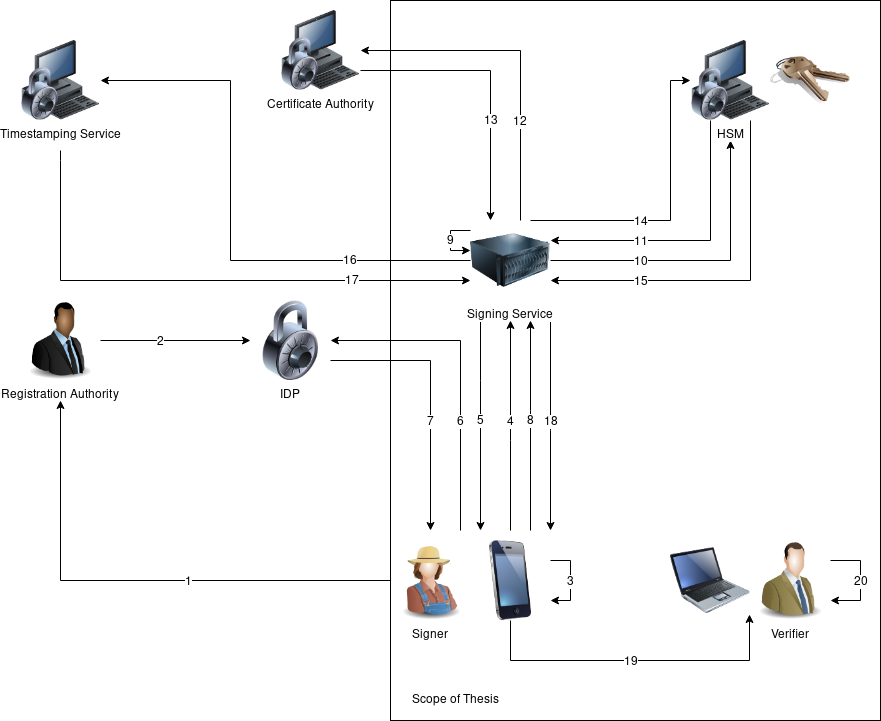
\includegraphics[scale=0.6]{images/BigPicture.png}
			\caption{Big Picture}
			\label{fig:bigpicture}
		\end{center}
	\end{figure}
	\vspace*{\fill}
\end{landscape}

\subsubsection{Steps}
\begin{enumerate}
	\item Registration of identity with RA (Authenticator)
	\item Propagate identity to IDP (Identifier)
	\item Generate document hash
	\item Send hash to signing service
	\item Receive OIDC redirect to IDP
	\item Login to IDP
	\item Receive ID token
	\item Send ID token to signing service
	\item Verify ID token
	\item Request signing key CSR from HSM
	\item Receive CSR
	\item Send CSR to CA
	\item Receive signed Certificate
	\item Request signature from HSM
	\item Receive signature
	\item Request timestamp from TSS
	\item Receive timestamp
	\item Send signature to signer
	\item Send document and signature to Verifier/Receiver
	\item Verify document and signature
\end{enumerate}


\section{The Signer}
\label{sec:actorsigner}
The Signer is the person who wishes to have the signing server sign a document in their name.
For example, a medical professional issuing a prescription for medication to a patient.

\section{The Verifier}
\label{sec:actorverifier}
The Verifier is the person who wishes to verify the integrity and authorship of a document.
For example, the pharmacist whom the patient gives the prescription to (as previously authored and signed by The Signer as specified in section~\ref{sec:actorsigner}) in order to purchase the medication prescribed by the medical professional.

\section{The Authenticator}
\label{sec:actorauthenticator}
The Authenticator is the system who authenticates The Signer as specified in section~\ref{sec:actorsigner}.
In \gls{NIST} terminology~\cite{nistdigitalidentityguidelines}, this is the entity establishing the \gls{IAL}.
In order for The Authenticator to be able to authenticate The Signer,
they must have been registered with The Authenticator by The Identifier as specified in section~\ref{sec:authoridentifier}.

\section{The Identifier}
\label{sec:authoridentifier}
The Identifier is the system or person who asserts the identity of The Signer.
In order for the signing service to issue qualified signatures as defined by relevant Swiss legislation~\cite{zertes} and Swiss Federal Council regulations~\cite{vzertes},
the identity must be proven in-person using a government-issued photographic identification document such as a passport.

\section{The Signing Service}
\label{sec:signingservice}
The Signing Service is the system who actually creates the signatures on behalf of the user.
It generates the signing keys and requests the \gls{CA}~\ref{sec:ca} to sign them.

\section{The Certificate Authority}
\label{sec:ca}
The \gls{CA} is the system who signs the signing keys generated by the Signing Service~\ref{sec:signingservice}.

\chapter{Functional Requirements}
\label{ch:functionalrequirements}

\section{Terminology}

As always, the usual modal verbs are to be interpreted as in RFC 2119~\cite{rfc2119}.

\subsection{Practically Impossible}
"Practically impossible" means the probability of it being possible is not zero, but so small for it not to matter in practice.
An example for this would be finding the prime factors of the product of two carefully chosen 1024 bit numbers within 24 hours.

\subsection{Being made difficult}
"Made difficult" means something far from impossible for someone with near-unlimited resources like a state actor,
but extremely difficult if not impossible even for a highly skilled single person with the resources expected for a single person.
For example, stealing a smart card from someone and misusing the contained private key.

\section{Signature Requirements}
\label{sec:signaturerequirements}
\subsection{Authenticity}
\label{subsec:authenticity}
It must be practically impossible for anyone to forge a signature without it being detected upon signature verification.

\subsection{Integrity}\label{subsec:integrity}
It must be practically impossible for anyone to modify a signed document without being detected upon signature verification.
A secure hash algorithm must be used for hashing the document.
Secure means the algorithm to be pre-image as well as collision-resistant as validated by the \gls{NIST} Cryptographic Algorithm Validation Program~\cite{nistcavp}.

\subsection{Verifiability}\label{subsec:verifiability}
Anyone must be able to verify the authenticity of a signature and the integrity of the signed document.

\subsection{Non-repudiation}\label{subsec:non-repudiation}
It must be practically impossible for anyone to deny having signed a document.

\subsection{Long-Term Validation}\label{subsec:long-term-validation}
Signatures must be suitable for \gls{LTV} using an RFC3161~\cite{rfc3161} timestamp.

\subsection{Secure Coupling of Authentication and Signature}\label{subsec:secure-coupling-of-authentication-and-signature}
It must be practically impossible for anyone to abuse a stolen \gls{OIDC} ID token to sign a document other than intended by The Signer.

\subsection{Authentication Protocol}\label{subsec:authentication-protocol}
Standard \gls{OIDC} must be used for authenticating The Signer as specified in the standard~\cite{oidc}.

\subsection{Supported File Formats}\label{subsec:supported-file-formats}
It must be possible to sign any file, regardless of its format.

\subsection{Bulk Signatures}\label{subsec:bulk-signatures}
For qualified signatures, it must be possible to sign more than one document at once.

For advanced signatures, it may be possible to sign several documents one after the other without requiring re-authentication.

\subsection{Device-local Hashing of Documents}\label{subsec:local-hashing-of-documents}
In order to ensure privacy and protection of information as required by~\ref{subsec:protection-of-information},
documents to be signed must not leave the users' device.
For webinterfaces, this means that the document must be hashed in the browser itself.

\section{Signature Server Requiremenents}
\label{sec:signatureserverrequirements}
\subsection{CA Key Security}\label{subsec:ca-key-security}
Technical measures must be taken to make it difficult for the private keys of the signing \gls{CA} to be stolen.

\subsection{Signing Key Security}\label{subsec:signing-key-security}
Technical measures must be taken to make it difficult to steal the private keys generated on behalf of the users.

\subsection{No unauthorised identity delegation}\label{subsec:no-unauthorised-identity-delegation}
It must be practically impossible for the signing server to create a signature on its own.

\subsection{Random Number Generation}\label{subsec:random-number-generation}
The \gls{RNG} used for generating signatures must be a cryptographically secure.

\subsection{REST API}\label{subsec:rest-api}
The Signature Server must offer a \gls{REST} \gls{API} that can be used by third parties to interface with the signing service,
for example in order to implement custom frontends or to include it as part of their product,
or for users that don't like \gls{GUI}s.

\chapter{Non-Functional Requirements}
\label{ch:nonfunctionalrequirements}

\subsection{Efficient Signature File Format}\label{subsec:efficient-signature-file-format}
The file format for the signature file shall be based on our previous work~\cite{projekt2}.

\subsection{Protection of Information}\label{subsec:protection-of-information}
Information not strictly required by the party in order to fulfil their function must not be disclosed to the aforementioned party.
In particular, the document to be signed must not be disclosed to the signing server nor to the \gls{IDP}.
The \gls{IDP} must not learn of the document hash.
More generally, every actor must not have any more information disclosed to it than is necessary for them to perform their function.

\subsection{Offline Validation}\label{subsec:offline-validation}
The Verifier must be enabled to verify signatures without an active internet connection using a desktop or laptop computer running GNU/Linux, MacOS or Windows.

\section{IDP Requirements}\label{sec:idp-requirements}
Anything related to the \gls{IDP} is out of scope for our thesis, except for specifying what we require of the same.
We assume to be using an existing, \gls{OIDC}-conforming \gls{IDP} providing the required registration and authentication levels.

\subsection{Support for OIDC}\label{subsec:support-for-oidc}
The \gls{IDP} must support standard \gls{OIDC} as specified in the standard~\cite{oidc}.


\subsection{Levels of Assurance}\label{subsec:levels-of-assurance}
The \gls{IDP} must support \gls{AAL} 2 authentication for advanced signatures, and \gls{AAL} 3 authentication for qualified signatures as specified in the \gls{NIST} publication~\cite{nistdigitalidentityguidelines}.

\section{Prioritisation of Requirements}
\label{sec:prioritisation}
\begin{longtable}{p{12cm}|p{2.5cm}}
    \textbf{Requirement} & \textbf{Prioritisation}\\
    \hline
    Authenticity of signature~(\ref{subsec:authenticity}) & Must\\
    Integrity of document~(\ref{subsec:integrity}) & Must\\
    Verifiability of signature~(\ref{subsec:verifiability}) & Must\\
    Non-repudiation~(\ref{subsec:non-repudiation}) & Must\\
    Secure coupling of authentication and signature~(\ref{subsec:secure-coupling-of-authentication-and-signature}) & Must\\
    Authentication protocol~(\ref{subsec:authentication-protocol}) & Must\\
    Supported file formats~(\ref{subsec:supported-file-formats}) & Must\\
    Signing key security~(\ref{subsec:signing-key-security}) & Must\\
    No unauthorised identity delegation~(\ref{subsec:no-unauthorised-identity-delegation}) & Must\\
    Random number generation~(\ref{subsec:random-number-generation}) & Must\\
    \gls{REST} \gls{API}~(\ref{subsec:rest-api}) & Must\\
    Offline validation~(\ref{subsec:offline-validation}) & Must\\
    Protection of information~(\ref{subsec:protection-of-information}) & Optional\\
    Device-local hashing of documents~(\ref{subsec:local-hashing-of-documents}) & Optional\\
    Efficient signature file format~(\ref{subsec:efficient-signature-file-format}) & Optional\\
    \gls{CA} key security~(\ref{subsec:ca-key-security}) & Optional\\
    Bulk signatures~(\ref{subsec:secure-coupling-of-authentication-and-signature}) & Optional\\
    Long-term validation~(\ref{subsec:long-term-validation}) & Optional\\
    \caption{Prioritisation of Requirements}
\end{longtable}

\chapter{Use-Cases}\label{ch:usecases}

\section{Document Signing}\label{sec:document-signing}

\subsection{Prerequisites}\label{subsec:prerequisites}
The following prerequisites have to be fulfilled in order for the following use cases to work:
\begin{enumerate}
    \item The user (actor~\ref{sec:actorsigner}) has registered with the \gls{RA} (actor~\ref{sec:authoridentifier}) and is known to the \gls{IDP}~(actor~\ref{sec:actorauthenticator})
    \item The user has created and readied a document file to be signed
\end{enumerate}

\subsection{Interactive Qualified Signatures}\label{subsec:interactive-qualified-signatures}
\subsubsection{Steps}
The user performs the following steps:
\begin{enumerate}
    \item Opens the webinterface of the signing service (actor~\ref{sec:actorsigningservice}) on their device
    \item Selects the document file to be hashed
    \item Selects the preferred \gls{IDP} out of a list of trusted \gls{IDP}s, if multiple \gls{IDP}s are configured
    \item Gets redirected to the \gls{IDP}s login page
    \item Authenticates with the \gls{IDP}
    \item Gets redirected back to the signing service
    \item Receives the signature as a file download
    \item Saves the signature file to their device
\end{enumerate}

\subsubsection{Result}
The user has received a signature file for the document file they wanted to sign.

\subsection{Bulk Advanced Signatures}\label{subsec:bulk-advanced-signatures}
In some cases, users might wish to sign document files all day long without being required to authenticate with the \gls{IDP} for every document.
In this case the authentication will be cached for a certain duration without needing to re-authenticate for each document.
In this mode only advanced signatures can be created.

From the users' point of view, it works like this:
\begin{enumerate}
    \item The user opens the webinterface of the signing service on their device
    \item If implemented, they click the button for authentication for batch advanced signatures
    \item Gets redirected to the \gls{IDP}
    \item Authenticates with the \gls{IDP}
    \item Gets redirected back to the signing service
    \item For the duration of the authentication, the user can now submit document files to be signed,
        receiving the corresponding signature files, without the need to reauthenticate.
\end{enumerate}
\subsubsection{Result}
The user receives advanced signature files for each of the document files they submit for signing for the duration of the authentication.


\section{Signature Validation}\label{sec:signature-validation}

\subsection{Prerequisites}\label{subsec:prerequisites2}
The following prerequisites have to be fulfilled in order for the following use cases to work:
\begin{enumerate}
    \item A signature file has been created beforehand as described in~\ref{subsec:interactive-qualified-signatures}.
\end{enumerate}

\subsection{Offline Validation}\label{subsec:offline-validation2}
The signatures can be verified offline with just the document file, the signature file and the verification program.
This mode will only be supported on desktop operating systems (GNU/Linux, Windows, macOS), not on mobile devices (Android, iOS).

\subsubsection{Steps}
The user performs the following steps:
\begin{enumerate}
    \item The user opens the verification program
    \item The user selects the document file and corresponding signature file and submits it to the verification program
    \item The program verifies the signature and displays the result
\end{enumerate}
\subsubsection{Result}
The user knows whether the signature is genuine and whether the document integrity is guaranteed.

\subsection{Online Validation}\label{subsec:semi-online-validation}
For mobile clients a website will be provided to validate the signature by providing the document and the signature.

\subsubsection{Prerequisites}
In addition to the prerequisites specified in subsection~\ref{subsec:prerequisites2},
it is necessary for the user to have opened the signature services' verification web page in their browser beforehand
so that it is available to the user without connecting to the server again.
This is why we call it semi-online.
For example, the user opens the web browser on their mobile phone and loads the verification page.
Then they board an aeroplane and turn on aeroplane mode.
After takeoff, they decide to validate a signature.
Then they proceed as follows:

\subsubsection{Steps}
The user performs the following steps:
\begin{enumerate}
    \item The user opens the web browser where the verification page is still available
    \item The user selects the document file and corresponding signature file and submits it to the verification website
    \item The website verifies the signature in-browser (without needing to connect to any additional servers) and displays the result
\end{enumerate}
\subsubsection{Result}
The user knows whether the signature is genuine and whether the document integrity is guaranteed.

\chapter{Project Management}
\label{ch:projectmanagement}

\section{Project Method}
\label{sec:projectmethod}
We will be using the SCRUM process for organising our work.
This means splitting the work packages into stories and scheduling for completion in sprints.
Sprints shall last two weeks. At the end of every sprint the progress is reviewed with the advisors and the next sprint is planned.

\section{Project Timeline}
\label{sec:projecttimeline}
Since we know in advance the timeframes within we must complete our work, we created the following project timeline.

\begin{landscape}
\topskip0pt
\vspace*{\fill}
	\begin{figure}[H]
	\begin{center}
		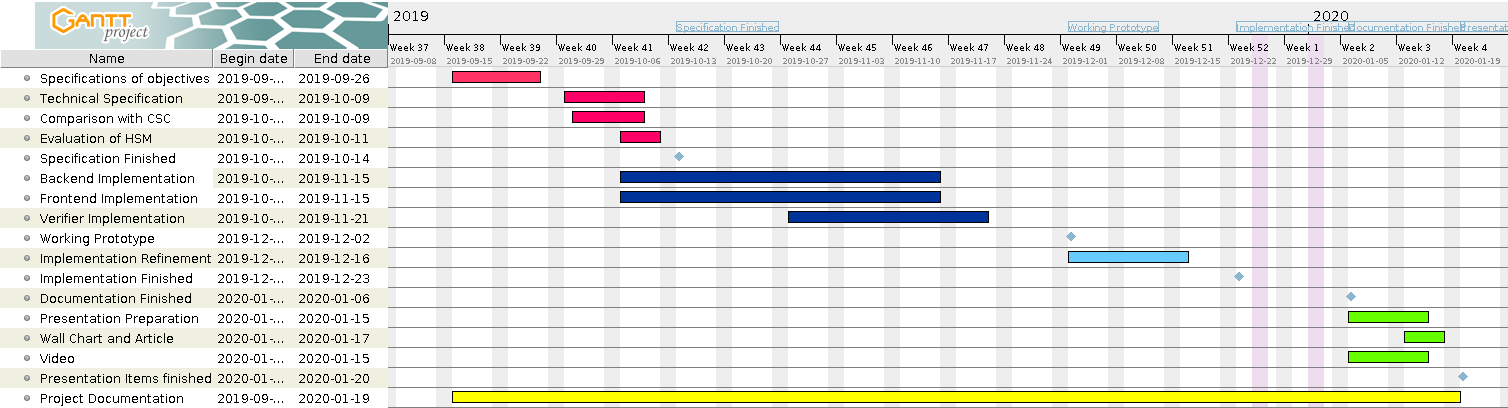
\includegraphics[scale=0.5]{images/Projectplan.png}
		\caption{Project timeline}
		\label{fig:projecttimeline}
	\end{center}
	\end{figure}
\vspace*{\fill}
\end{landscape}

\section{Work Packages}
\label{sec:workpackages}

\subsection{Specification of Objectives}\label{subsec:specification-of-objectives}
The objectives of our thesis will be specified.
This included functional and non-functional requirements.

\subsection{Technical Specification}\label{subsec:technical-specification}
The requirements defined in the objectives will be mapped to concrete technology choices.
Also the choice of languages and frameworks will be explained.

\subsection{Comparison with CSC Implementation}\label{subsec:comparison-with-csc-implementation}
We will compare our Specification with the Remote Signing Standard specified by the \gls{CSC}.

\subsection{Evaluation of Yubikey HSM}\label{subsec:evaluation-of-yubikey-hsm}
We will evaluate how we can use the Yubikey HSM for our Signature Service.

\subsection{Backend Implementation}\label{subsec:backend-implementation}
The backend consisting of the Signing Service and the OIDC Coupling with the IDP will be implemented.

\subsection{Frontend Implementation}\label{subsec:frontend-implementation}
The frontend consisting of the Hashing and UI will be implemented.

\subsection{Standalone Verifier Implementation}\label{subsec:standalone-verifier-implementation}
The application for the offline verification of the signature will be implemented.

\subsection{Implementation Refinement}\label{subsec:implementation-refinement}
After the working prototype, eventual bugs will be fixed and optional goals will be implemented.

\subsection{Source Code Documentation}\label{subsec:source-code-documentation}
We will document the source code.

\subsection{Presentation}\label{subsec:presentation}
We will create the slides and prepare the presentation.

\subsection{Wall Chart and Article}\label{subsec:wall-chart-and-article}
We will create a wall chart and short article describing our work.

\subsection{Video}\label{subsec:video}
We will create a short video introducing our problem.

\part{Report}
\chapter{Introduction}
\label{ch:Introduction}

The trend for Signing Service Solutions goes in the direction of Remote Signing.
Users no longer hold on to the cryptographic keys themselves,
instead a remote service stores the users' signing keys or even generates the keys on-demand.
This has a serious drawback:
such a signing service is able to sign without user's knowledge or consent,
thus it must offer complete trustworthiness.
In this thesis,
we provide a specification as well as a proof-of-concept where the signing process is tied to the identity of the user,
such that the signing service by itself cannot sign a document.

The implementation consists of the remote signing service itself exposing a \gls{REST} \gls{API},
a cross-platform verification program offering both online and offline verification,
and a cross-platform frontend authenticating the users through a trusted \gls{OIDC} \gls{IDP}.


\section{Previous Works}
\label{sec:previousworks}

We build upon our previous work of Project 2~\cite{projekt2},
where we specified the authentication process for qualified signatures,
non-qualified batch signatures,
a signature file format,
as well as - to our knowledge - pioneering the secure integration of a digital signature with an \gls{OIDC} ID token without requiring any change to the \gls{IDP}.

In this thesis, we expand upon our previous work substantially both functionally and conceptually.
This thesis is not just an implementation of an existing concept.

\section{Overview of Contents}\label{sec:overview}
TODO


\section{A cryptographic primer}\label{sec:a-cryptographic-primer}
In this section we well very briefly introduce the most important IT security and cryptography building blocks we use to make remote digital signing possible.
Readers with a basic knowledge of IT security topics such as hash functions, X.509, \gls{PKI} and \gls{DSA} can safely skip it.
The descriptions given are as brief as possible in order to introduce the topics, they're not meant to be complete nor excruciatingly precise.

\subsection{Hash Function}\label{subsec:hash-function}
A hash function in cryptography is an one-way function which is able to map data of arbitrary length to fixed-size values~\cite{hashing}.
One-way means that for a given hash value, it is infeasible to find the corresponding input data.
Ideally, the only way for someone to invert such a hash function is to do an exhaustive brute-force search.
This is called pre-image resistance.
Furthermore, a cryptographic hash function needs to fulfil the following properties:
\begin{enumerate}
    \item For a given input value, it must always produce the same hash value (it must be deterministic)
    \item It must be infeasible to find to different input values that produce the same hash value (this is called collision resistance)
    \item For a given input value, it must be infeasible to find another input value that produces the same hash value (second pre-image resistance)
    \item A minimal change in the input value must result in a completely different output value (avalanche effect)
\end{enumerate}

Hash functions fulfilling these properties are fundamental to our work (and to much of cryptography in general).
Without them we would be completely powerless.
An example for such a hash function is \gls{SHA-2}~\cite{sha2patent}.

\subsection{Asymmetric cryptography}\label{subsec:asymmetric-cryptography}
Asymmetric cryptography, sometimes called public-key cryptography, is a type of encryption which uses pairs of keys.
This is in contrast to symmetric encryption which uses only one key (for example, a passphrase encrypting a file).

With symmetric encryption the passphrase must me known both to encrypt and to decrypt the message,
but with public-key cryptography, the public key can be used to encrypt a message and the private key to decrypt it.

This might sound simple on the surface but opens up a world of possibilities.
Only the private key has to be kept secret, the public key can be freely published~\cite{stallings}.

The classical example for such an encryption system is the \gls{RSA} scheme~\cite{rsa}.

For a simplified example how public-key-based encrypted communication between two parties could work,~\footnote{
We're well aware of the major security problems in this example,
like the fact that both the key exchange and the message exchange happen unauthenticated and without integrity protection,
but we intentionally chose to keep the example as simple as possible in order to keep it easily comprehensible by a wide audience.
}
see figure~\ref{fig:simplepubkeycomm}.

\begin{figure}
    \centering
    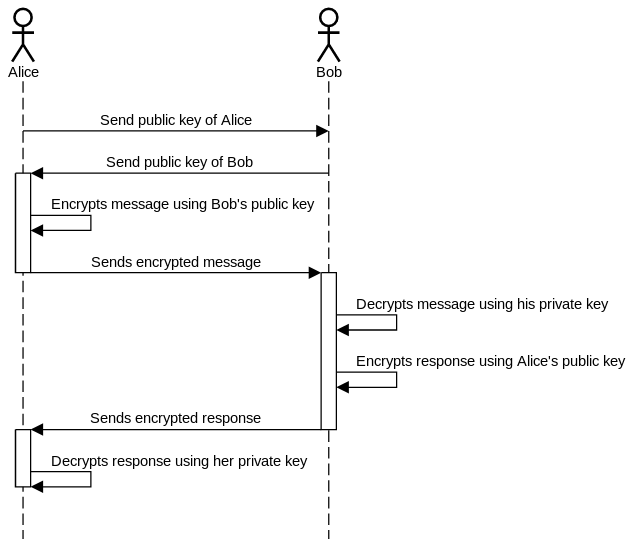
\includegraphics[width=0.75\textwidth]{images/simplistic_pubkey_communication.png}
    \caption{Simplified example of two Actors, Alice and Bob, exchanging encrypted messages using public-key cryptography}
    \label{fig:simplepubkeycomm}
\end{figure}


\subsection{Digital Signatures}\label{subsec:digital-signatures}
Having briefly explained Hash Functions in~\ref{subsec:hash-function} and Asymmetric Encryption in~\ref{subsec:asymmetric-cryptography} we can now move on to introducing digital signatures.
A digital signature is a way for verifying the integrity and authenticity of a message, that is,
to know who the message author is and to guarantee that it wasn't tampered with~\cite{digitalsignature}.

\paragraph{Digital Signatures are not Electronic Signatures}
Please note that the Digital Signatures we describe here are distinct from Electronic Signatures.
Electronic signatures provide the same legal standing as a hand-written signature on paper,
and as such are defined in laws such as ZertES~\cite{zertes}.
Digital signatures on the other hand merely refer to a mathematical scheme for providing message integrity and authenticity.
Digital signatures are used to implement electronic signatures, but they're not equivalent.


If we want to create a digital signature on a message, we perform the following steps:
\begin{enumerate}\label{enum:digitalsignaturecreation}
\item We take our message and run it through a cryptographic hash function, thus obtaining the hash value.
\item Then, we encrypt the hash value using our private key.
\item We transmit the message and the encrypted hash value to the recipient.
\end{enumerate}

In order to verify the authenticity and integrity of the message, the recipient performs the following steps:
\begin{enumerate}
    \item They run the message through the same cryptographic hash function we did and obtain its hash value.
    \item They decrypt the encrypted hash value we sent them using our public key and compare it to the hash value they obtained themselves in step 1.
    \item If the values match, the recipient can be confident that a) the message wasn't tampered with and b) we authored it.
\end{enumerate}

In the message exchange shown in figure~\ref{fig:simplepubkeycomm},
there is a problem: anyone could encrypt messages for Bob and pretend to be Alice, since his public key is, well, public.

So by employing public-key cryptography, Bob is able to receive encrypted messages from Alice but they're of limited use to him,
since he has no way of knowing who actually sent them.
Fortunately, we can solve this problem by using digital signatures.

Before Alice encrypts her message to Bob using his public key,
she creates an digital signature by using a hash function and her private key as described above.
Then she encrypts both the message and the signature using Bobs public key and sends the two to him.

Bob then decrypts the message and verifies the digital signature as described above.

However, there is a serious problem still: an evil actor with the ability to intercept the communication
between Alice and Bob could not only read their messages,
but change them at will, effectively impersonating Bob as seen from Alice,
and Alice as seen from Bob.
For a solution to this problem please see section~\ref{subsec:digital-signatures}.

Figure~\ref{fig:pubkeymidm} expands upon figure~\ref{fig:simplepubkeycomm} to illustrate this attack.

\begin{figure}
    \centering
    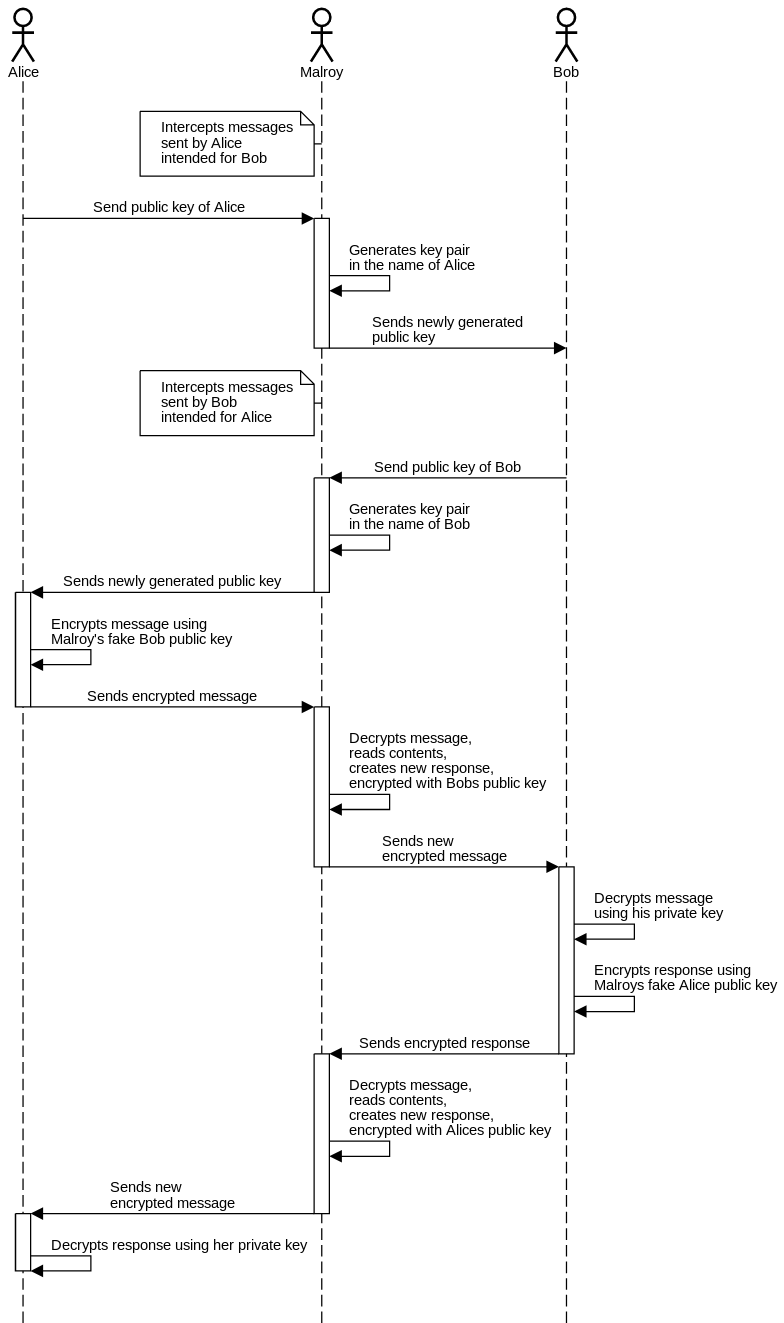
\includegraphics[width=0.85\textwidth]{images/pubkey_midm.png}
    \caption{Man in the middle attack on unauthenticated public-key encrypted communication}
    \label{fig:pubkeymidm}
\end{figure}


\subsection{Public-Key Infrastructure and Certificate Authorities}\label{subsec:public-key-infrastructure-and-certificate-authorities}
Public-key encrypted and authenticated communication as described in chapter~\ref{subsec:digital-signatures}
is vulnerable to man-in-the-middle attacks as illustrated in figure~\ref{fig:pubkeymidm}.
This attack works because Malroy is able to mislead Bob and Alice to use his keys instead of theirs
by intercepting their public keys in the initial key exchange.

This could be solved trivially if Alice and Bob exchanged their keys in a secure manner,
for example by meeting face-to-face,
thus ensuring Malroy can't sit in the middle.
However, this negates the main advantage of using public-key cryptography:
if they're forced to meet they could just as well exchange a symmetric key and use that for encrypting
their messages.

This one of the problems a \gls{PKI} solves.
On an abstract level, a \gls{PKI} is a mechanism that couples a public key with an identity~\cite{whatispki}.
What this means for the attack shown in figure~\ref{fig:pubkeymidm} is that it provides Alice and Bob
a way to make sure they're using each others' keys and not Malroys',
thus preventing the attack.
Because Alice and Bob now have a mechanism to verify which identity a public key refers to,
they can detect Malroys attack because the public keys maliciously issued by him will not correspond to Alice nor Bob.

A well-known and widely-used example for such a \gls{PKI} is X.509~\cite{x509}.
In practice such \gls{PKI}s are complex,
and because this section's already become longer than we like we'll forego explaining how X.509 works.

\subsection{Trusted Digital Timestamping}\label{subsec:timestamps}
Trusted digital timestamping is a scheme for proving the existence of a piece of information at a certain point in time.
There are several such schemes, such as X9.95 or ISO/IEC 18014.
In this section we will focus on \gls{PKI}-based timestamping as defined in RFC 3161~\cite{rfc3161}.

In RFC 3161, timestamps are issued by a trusted third party, the \acrfull{TSA}.

Trusted timestamps are created by using digital signatures (see~\ref{subsec:digital-signatures}) and hash functions (see~\ref{subsec:hash-function}).
In order to create a timestamp, the following steps are performed:
\begin{enumerate}
    \item We feed the information to be timestamped to a hash function and obtain its the hash value
    \item We send the hash value to the \gls{TSA}
    \item The \gls{TSA} concatenates the hash value with a timestamp
    \item The \gls{TSA} feeds the concatenation of our hash value with the timestamp to a hash function, in turn obtains the hash value of the concatenation
    \item The \gls{TSA} digitally signs the hash value from the previous step
    \item The \gls{TSA} sends the signed hash as well as the timestamp back to us
    \item We store the signed hash, the timestamp and the original information
\end{enumerate}
For an illustration of this process, see figure~\ref{fig:timestamping}

\begin{figure}
    \centering
    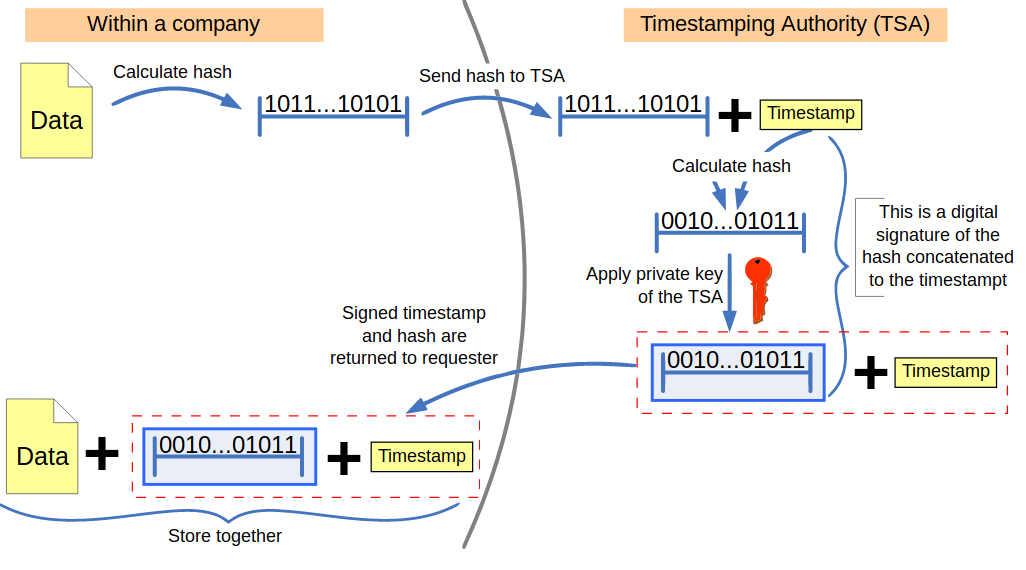
\includegraphics[width=0.85\textwidth]{images/timestamping.png}
    \caption{Process of obtaining a timestamp from a \acrfull{TSA}.
    Source: \url{https://en.wikipedia.org/wiki/File:Trusted_timestamping.svg}}
    \label{fig:timestamping}
\end{figure}

\subsection{Summary}
In a nutshell, the main ideas to take away from this chapter are:
\begin{itemize}
    \item Hash functions are one-way functions, mapping data of arbitrary length to fixed-length values
    \item Asymmetric cryptography allows for advertising the public portion of the key, and can be used to encrypt messages
    \item Digital signatures provide a means of verifying the integrity and authorship of a message
    \item Public Key Infrastructures provide a way to pair a public key with an identity
    \item Trusted Digital Timestamping is a means to proving the existence of a piece of information at a given point in time
\end{itemize}

\chapter{Evolution of the Signing Protocol}
\label{ch:signingprotocol}

\section{Overview}
The purpose of the signing protocol is to specify which steps have to be carried out by which actor in what
order so as to create a signature.

\section{Signature Format}
\label{sec:signatureformat}

When using our signing service, people should be able to sign arbitrary files of any format.
We don't want to place restrictions upon users such as "\gls{PDF} only" or "Microsoft Word documents only".
Such restrictions are unnecessary and would only serve to constrain the number of people using the service
(as they couldn't use their preferred formats).

This requirement presents us with a small challenge,
since it is impossible to embed a digital signature into arbitrary file formats.
Some formats support it out of the box, such as \gls{PDF}~\cite{etsipades},
while with others existing metadata fields could be repurposed to contain signature data.
Finally with some formats it's not possible to include additional data at all.

The government of Estonia faced the same problem when they developed their solution to digital signatures.
They solved it by creating a new document format called DigiDoc~\cite{digidoc},
which, in essence, is a container format for the actual document along with the signature information.
With their solution, arbitrary document formats can be used,
but the downside is that the user needs to install a program that is able to extract and display the document contained in DigiDoc,
even if they just wished to view the document without verifying the signature.

For this reason, we chose to have a detached signature file, that is,
the signature data resides in a file separate from the document that was signed.
In contrast to the Estonian solution,
the advantage is that people don't need to install additional software if all they want is to view the signed document.
The disadvantage is that users need to handle two files instead of one (the document and its signature).


\subsection{Original Format}\label{subsec:original-format}
Our original specification for the signature format is based on our work in Projekt 2~\cite{projekt2} which contained the following fields:

\begin{itemize}
    \item Signature (Base64)
    \item Signature format (\gls{RSA-PSS}, \gls{Ed25519})
    \item Signature hash algorithm (\gls{SHA}256, \gls{SHA}3)
    \item Timestamp according to \gls{RFC} 3161\footnote{\url{https://tools.ietf.org/html/rfc3161}}
    \item Public key (\gls{PEM})
    \item Issuing \gls{CA} (\gls{PEM})
    \item Subject
    \item Validity
    \item Level
\end{itemize}

This format would be encoded as a protobuf message in order to not have an overly verbose file (as opposed to \gls{XML}),
but still support having a schema (as opposed to \gls{JSON}).

\subsection{Difference Between Advanced And Qualified Signatures}\label{subsec:difference-between-advanced-and-qualified-signatures}
The distinction between electronic and digital as well as advanced and qualified signatures is derived from Swiss Federal Law~\cite{zertes}.

\subsubsection{Electronic or Digital Signatures}
An electronic signature is a purely technical, non-legal term.
Put simply, the term denotes electronic information associated logically with other electronic information.
Such information may be used by a signatory for creation of a signature.
It may simply consist of a digitally scanned, handwritten paper signature.

In contrast, a digital signature is always based upon one or several cryptographic algorithms.
A digital signature incorporates an unforgeable representation of the original data (guaranteed integrity)
and, as such, enables proof of the origin of data.

\subsubsection{Advanced Electronic Signature}
As defined in Swiss Federal Law~\cite[Art. 2]{zertes},
an advanced electronic signature is an electronic signature which fulfills the following requirements:

\begin{enumerate}
    \item It is exclusively associated with the holding person
    \item It allows for identification of the holding person
    \item It is created by means under sole control of the holding person
    \item It is associated with personal information of the holding person in such a manner that retroactive modification of the data can be detected
\end{enumerate}

Advanced electronic signatures have no direct legal significance, however,
they may reinforce the cogency of proof in a court of law~\cite[4.19]{crypto-folien-hassenstein}.

\subsubsection{Qualified Electronic Signature}
A qualified electronic signature is an advanced electronic signature which meetds the following additional conditions:
\begin{enumerate}
    \item It is created using a secured signature creation device~\cite[Art. 6]{zertes}
    \item It is based upon a qualified certificate~\cite[Art. 7 and 8]{zertes}, whose subject is a natural person,
    and which was valid at the time of signature creation.
\end{enumerate}

A qualified electronic signature is legally equivalent to a hand-written signature, that is,
it is admissible in a court of law, it can be used to sign legally binding contracts, and so on.


\section{Flaws of the Original Protocol}\label{sec:flaws-of-the-original-protocol}
The original protocol, which we specified in Projekt~2~\cite{projekt2} employed a server-side secret nonce to generate the nonce used in the \gls{OIDC} authentication request,
which needed to be kept in memory until the signer returned with the ID token from their trip to the \gls{IDP}.
This could be abused to \gls{DoS} the signing server, and it made this part of the signing server stateful.

Furthermore,
for the verification of the signature all documents that were signed together needed to be present at the time of verification,
since their hashes were incorporated in the \gls{OIDC} nonce.

Moreover, multi-signatures, while technically possible, were made impractical for some applications:
If a single person wishes to sign multiple documents at once that will be used together,
(for example, an apartment rental contract, house rules, and a bank deposit confirmation)
this won't be a problem.
However, if multiple, independent documents are to be signed together
(for example, a company sending 50 bills to 50 different customers),
having to send each customer all the bills is just silly.

\subsection{Draft 1: Making the Protocol stateless}\label{subsec:draft-1:-making-the-protocol-stateless}
Since storing the secret nonce on the signing server is undesirable,
we thought about changing the protocol to make this part stateless.

To achieve this, we introduce two more nonce-like values called \texttt{seed} and \texttt{salt}.
The \texttt{seed} is a randomly generated value that is used to verify the id token when the signer returns from the \gls{IDP}.
The \texttt{salt} is the \gls{MAC} of the document hash(es) concatenated with the \texttt{seed}, using a static server side secret as key.

The \texttt{salt} takes the role of the original nonce that was used to construct the \gls{OIDC} nonce and protects against the \gls{IDP} gaining knowledge of the signed hashes and to protect against the \gls{IDP} learning about the document hashes.

The signing server returns both the \texttt{seed} and the \texttt{salt} to the client,
which then constructs the \gls{OIDC} nonce.
The \gls{OIDC} nonce is now the \gls{MAC} of the list of hashes with the \texttt{salt} used as key.

When the signer returns to the signing server, it presents the \texttt{seed}, \texttt{salt}, the hashes and ID token.
Using the \texttt{seed} and the static secret the server can reconstruct the \texttt{salt} and verify that the presented \texttt{salt} is the same.

This functions as a \gls{CSRF} protection of a malicious \gls{IDP} requesting signatures using past values,
while also allowing us to keep the signing server stateless.

After this step the \texttt{seed} will not be used anymore and therefore doesn't need to be in the signature document.
The \gls{OIDC} token will then be verified with the \texttt{salt} and the hashes.

\subsection{Draft 2: Improving signing of multiple documents}\label{subsec:draft-2:-improving-signing-of-multiple-documents}
Even with the improvements in draft 1 (section~\ref{subsec:draft-1:-making-the-protocol-stateless}),
only one signature file will be generated for multiple documents, incorporating all document hashes irrevocably linked together.
Verifying the signature would require having all documents present, which is impractical.

To solve this, our first idea was to include the hashes of the other documents, signed together,
and then generate a signature for each file.
The sorted list of hashes is fed to the \gls{MAC} function in the verification step.
This however would leak information about the other documents, as they would be just plain hashes.
We put a lot of thought into minimising the amount of information all involved actors learn,
such as masking the document hash from the \gls{IDP}, and we're not satisfied with a solution where the other recipients learn
about unrelated document hashes just because they were signed together.

Our solution for this is to generate a \gls{MAC} of each hash with the \texttt{salt} as key and include that in the signature file,
with the \gls{OIDC} nonce just being the hash of the sorted \gls{MAC}s.

This way the verifiers' own \gls{MAC} can be generated during verification with the other \gls{MAC}s just being used as additional input parameters without leaking the hashes of the documents.
Assuming the \gls{HMAC} function used is secure,
the only information that the receiver of the signature file could learn is the number of the documents that were signed together.

\subsection{Draft 3: Simplifying and using CMS where possible}\label{subsec:draft-3:-simplifying-and-using-cms-where-possible}
Draft 2 (section~\ref{subsec:draft-2:-improving-signing-of-multiple-documents})
resulted in a rather complicated schema that looked something like listing~\ref{lst:draft2schema1}.

\begin{lstlisting}[caption={Draft 2 schema 1}, captionpos=b, label={lst:draft2schema1}]
    message SignatureData {
    bytes document_hash = 1;
    HashAlgorithm hash_algorithm = 2;
    bytes mac_key = 3;
    MACAlgorithm mac_algorithm = 4;
    repeated bytes other_macs = 5;
    SignatureLevel signature_level = 6;
    bytes id_token = 7;
    repeated bytes jwk_idp = 8;
    map<string, LTV> ltv_idp = 9;
    }

    message Timestamped {
    bytes rfc3161_timestamp = 1;
    map<string, LTV> ltv_timestamp = 2;
    }

    message SignatureContainer {
    bytes enveloped_signature_data_pkcs7 = 1;
    map<string, LTV> ltv_signing = 2;
    }

    message LTV {
    bytes ocsp = 1;
    bytes crl = 2;
    }

    message SignatureFile {
    SignatureContainer signature_container = 1;
    repeated Timestamped timestamps = 2;
    }
\end{lstlisting}

\texttt{SignatureData} is the information that gets signed.
It obviously contains the hash of the document in \texttt{document\_hash},
but for the reasons explained in~\ref{subsec:draft-2:-improving-signing-of-multiple-documents}
we need to include the other maskes hashes: that's what \texttt{other\_macs} is for.

\texttt{Timestamped} allows us to add certificate revocation information (\gls{CRL} and \gls{OCSP}) for the certificates used in the RFC~3161~\cite{rfc3161} timestamps.
The inclusion of these is necessary for proper offline verification, where the verifier is most likely not able to retrieve this information by itself.

\texttt{SignatureContainer} is used to add revocation information for the certificates used in \texttt{SignatureData}.

When we examined RFC~5652~\cite{rfc5652} more closely, we discovered that it's possible to add
\gls{CRL}s as well as \gls{OCSP} responses to \gls{CMS} messages (but not to \gls{PKCS7}~\cite[Section 10.2.1, RevocationInfoChoices and OtherRevocationInfoFormat]{rfc5652}).
Since both \texttt{SignatureData} and the RFC~3161~\cite{rfc3161} timestamps are RFC~5652~\gls{CMS} messages which do support including revocation information,
we can simply put the revocation information in there and don't need our own message formats.

Then it occured to us that we don't need to have the hash of the current document separate from the masked hashes of the other documents.
We can simply include a list of masked hashes.

This works, because during verification, the original documents are present.
The verifier simply calculates their hash values, masks the hashes using \texttt{mac\_key},
and checks whether they're present in the list of masked hashes.
This slightly simplifies the verification process,
but the main advantage of this change is that it speeds up issuance of multi-file signatures tremendously.

When before, we created a signature file per document hash, now we create one signature file for all documents signed together.
Since creating a signature file entails a nontrivial amount of work this change represents a vast improvement in signature creation speed.

\begin{lstlisting}[caption={Simplified schema}, captionpos=b, label={lst:draft2schema2}]
    message SignatureData {
    repeated bytes salted_document_hash = 1;
    HashAlgorithm hash_algorithm = 2;
    bytes mac_key = 3;
    MACAlgorithm mac_algorithm = 4;
    SignatureLevel signature_level = 5;
    bytes id_token = 6;
    bytes jwk_idp = 7;
    map<string, LTV> ltv_idp = 8;
    }

    message LTV {
    bytes ocsp = 1;
    bytes crl = 2;
    }

    message SignatureFile {
    bytes signature_data = 1;
    repeated bytes rfc3161 = 2;
    }
\end{lstlisting}


Unfortunately we can't get rid of \texttt{LTV} completely because there is no way to add revocation information
to a RFC~7517~\cite{rfc7517} JWK, so we still need it for the \gls{IDP} certificates.
Still, these changes result in a significant simplification of the schema, as seen in listing~\ref{lst:draft2schema2}.


\chapter{Technical Specification}
\section{REST API}
TODO
\section{Signature File Format}
TODO
\subsection{Long-Term Verification}
Long-term signature validation allows for validation of signatures long after the document was signed~\cite{etsipades}.
In order for us to achieve this, all required elements for signature validation must be embedded into the signature file.
Without the addition of these elements, a signature can only be validated for a limited time.
This limitation occurs because the \gls{CA}s eventually expire or are revoked.
Once the \cls{CA} certificate has expired, the issuing authority is no longer responsible for confirming the revocation status on that certificate.
Without the confirmed revocation status information, the signature cannot be validated.

To overcome this limitation, the following information has to be embedded into the signature:
\begin{enumerate}
    \item The signing certificate
    \item A timestamp on the signature
    \item The certificates used and their revocation status (\gls{OCSP} and \gls{CRL})
    \item An archive timestamp of the previous content
\end{enumerate}

The archive timestamp establishes the date in which the information collected was issued.
Provided the archive timestamp is valid,
we can trust the revocation information was issued at that time and check the validity of the signing certificate and the \gls{CA} certificate chain,
and be sure that it was not revoked at the point in time the document was signed.
This allows us to extend the validity of the signature past the expiration time of the \cls{CA}.

However, this does not extend the validity of the signature indefinitely,
it merely extends the expiration until the expiration time of the timestamp certificate.
When the timestamp certificate is close to expiration,
the signature expiration time has to be extended by adding another timestamp signed by a certificate not close to expiration.
This process has to be repeated periodically in order to keep the signature valid and verifiable.


\chapter{Implementation}
\section{Choices in Technologies}
\label{sec:techchoices}
In this chapter, we outline the technologies we choose, and the reasoning for choosing them.

\subsection{Backend}
\label{subsec:techbackend}
The backend is divided into two parts, the signing service and the verification service.
They are developed independently in different programming languages.

We chose to split the backend into two because signature verification has to be available both online and offline.

Using two different programming languages and sets of libraries,
implementing common formats and protocols independently from specification alone,
allows us to hedge against the risk of some flaws in the libraries: if a library used in the signing service produced flawed output,
it would likely be discovered by the verification service since it uses a different implementation of the same concepts.
The exact same flaw being present in two different libraries implemented in different programming languages is rather small.

On top of that, we can test ourselves how well we've specified the protocols and formats:
if these two services can be used together without problems, the specification was precise enough.
If not, we learn where we must improve it, which is a win-win situation.

\subsubsection{Signing Service}
The signing service is implemented in the Kotlin programming language~\cite{kotlin} using the Ktor framework~\cite{ktor}.
For the signing service we chose Kotlin because it is a modern and concise programming language,
providing null safety, coroutines for asynchronous programming,
support for functional programming with higher-order functions and closures,
and it's genuinely nice to program in.
Kotlin offers seamless Java interoperability, allowing us to make use of the excellent and extensive Java ecosystem.

We haven't picked Kotlin and Ktor at random, we've discussed which language and framework to use for the signing server at length.
The table~\ref{tab:langandfram} lists a short overview which other choices we've discussed but chosen not to pursue.

\begin{figure}
    \begin{center}
        \begin{tabular}{p{1.5cm}|p{2cm}|p{11cm}}
            \textbf{Language} & \textbf{Framework} & \textbf{Reason for non-consideration} \\
            \hline
            Java & Spring MVC & Steep learning curve, vast amount of functionality to learn, too large for our needs, little previous knowledge on our part \\
            \hline
            Java & Vaadin & Generated frontend is slow to use because of network latency, too much uncertainty with regards to \gls{WASM} integration: Is it possible? How? How long will it take us, how much will we have to implement ourselves? \\
            \hline
            C\# & .NET Core & Zero previous knowledge on our part both for the language and the framework, aversion to Microsoft because of their attempts to undermine open-source software~\cite{mseee} \\
            \hline
            Scala & Play & Little previous knowledge of the language, uncertainty of the time required to learn it properly, but otherwise an interesting contender \\
            \hline
            Python & Django & Huge framework to learn, no type safety, slow runtime performance \\
        \end{tabular}
        \captionof{table}{Programming languages and frameworks considered for use in the signing service implementation\label{tab:langandfram}}
    \end{center}
\end{figure}


\subsubsection{Verifier}
The verification service is implemented in the Go programming language~\cite{golang}.
For the verifier we chose Go,
because it allows us to generate statically linked binaries for all major platforms,
without worrying about dependencies.
Further the Go standard library already includes a lot of cryptographic functionality,
requiring fewer third party dependencies.
Go's built-in concurrency primitives (goroutines and channels) make it easy implement the verification of the many parts of the signatures asynchronously.
With only having a single \gls{API} endpoint for verifying the signature it isn't necessary to use a complicated web framework as the \texttt{http} package of the Go standard library provide all needed functions.

As with the signing service implementation, we evaluated alternatives, which are summarised in table~\ref{tab:goalts}.

\begin{figure}
    \begin{center}
        \begin{tabular}{p{1.5cm}|p{2cm}|p{11cm}}
            \textbf{Language} & \textbf{Framework} & \textbf{Reason for non-consideration} \\
            \hline
            Java & JavaFX & Requires the user to either have Java installed or will be bundled with the program, which makes it quite large.  \\
            \hline
            Anything & Electron & Electron is ludicrously resource-hungry, having the Chromium engine underneath. It also requires more frontend (javascript) code than any of us is comfortable with. \\
        \end{tabular}
        \captionof{table}{Programming languages and frameworks considered for use in the verification service implementation\label{tab:goalts}}
    \end{center}
\end{figure}


\subsection{Frontend}
\label{subsec:techfrontend}

Given that the frontend must support the three desktop operating systems Microsoft Windows,
GNU/Linux as well as Apple MacOS,
the technological choices available to us are limited.
On the desktop, we could use the \gls{JVM} platform and the JavaFX \gls{GUI} library, whereas on the phones
we could use Flutter~\cite{flutterframework}.
However, developing three applications on five platforms using two new-to-us frameworks and programming languages
would take a lot more time and resources than what is available to us in the scope of this thesis.

In order to reduce complexity and enable code reuse, we decide to implement the frontend as a web application.
Web frontents are capable of running in any modern web browser regardless of platform, be it mobile or desktop.
We're not happy about this, as we would much rather use mature, strongly-typed and well-designed languages and frameworks,
but we're forced to make this compromise in order to meet our objectives in the time available.
In order to reduce the pain, we will use TypeScript, which is a typed superset of JavaScript~\cite{loltypes}.
We discussed implementing a \gls{SPA} using Angular~\cite{angular},
but for our use case it's overkill as there isn't too much client-side logic.
In the interest of a small, fast-loading site we chose to stick with plain \gls{HTML} and \gls{CSS}
and only adding as much JavaScript as necessary.

\subsection{Client-Side File Hashing in the Web Browser}
\label{subsec:browserhashing}
However, the decision to implement the frontend as a web application presents us with a challenge:
hashing the files to be signed client-side in the web browser itself.
If we had implemented "proper" client applications this would've been easy, but in a web browser and using its
JavaScript language not so much: it simply wasn't designed with performance in mind.

The easiest solution would be to upload the files to be signed to the server and hash them there,
but this would be a clear violation of the least-information principle (the server doesn't need the file, only the hash)
and a breach of user privacy.
Nevermind the fact that signing large files could take a very long time over slow network connections,
and turn out to be quite expensive for mobile users billed for data by volume.

Another solution would be to ask the user to enter the file hashes instead of selecting files,
but this would be very user-unfriendly and most likely too much to ask from many users.

It is clear we must find a way to hash files in the web browser itself.
In order to achieve this we have found the following options:

\begin{enumerate}
    \item Using the browser-implemented \texttt{SubtleCrypto}~\cite{subtlecrypto} \gls{API}
    \item Using the \texttt{CryptoJS}~\cite{cryptojs} JavaScript implementation
    \item Using a \gls{WASM}-based implementation
\end{enumerate}

Each of these options comes with a number of advantages and disadvantages, as discussed in more detail in the following sections.

\subsubsection{Using SubtleCrypto}
\label{subsec:subtlecrypto}
The \texttt{SubtleCrypto} class offers the \texttt{digest(algorithm, data)} method~\cite{subtlecrypto}, which can be used to
calculate \gls{SHA-256} checksums.
The advantage of using this implementation is that it is available in all modern browsers\footnote{Where modern browsers means Mozilla Firefox, Google Chrome/Chromium, and Microsoft Edge, not older than the respective versions available in 2018},
and since it's executed with native code, being able to take advantage of \gls{AVX2} instructions, instead of JavaScript it should be quite fast.
There's a major drawback though: hashing a large amount of data progressively is not supported, the data has to be
passed to the function en bloc, as seen in listing~\ref{lst:subtlecrypto}.

\lstinputlisting[caption={Using SubtleCrypto for calculating SHA-256 checksums}, captionpos=b, language=JavaScript, label={lst:subtlecrypto}]{listings/subtlecrypto.js}

Our testing showed that selecting files larger than 200MB crashes Firefox tabs when trying to read their contents
into memory before we could pass it to the \texttt{digest} function.
If we assume the users will only ever select small files this should not pose a problem, but unfortunately it's not safe to assume this.
Furthermore, this limit is probably lower still on mobile devices such as smartphones (although we didn't test this).

\subsubsection{Using CryptoJS}
\label{subsec:cryptojs}
\texttt{CryptoJS} does not have the limitation of \texttt{SubtleCrypto} and supports progressive hashing\footnote{
By progressive hashing we mean the ability to pass to the hash function the data piece by piece in order to avoid holding all of it in memory at once.},
as seen in listing~\ref{lst:cryptojsprogressive}.

\lstinputlisting[caption={Progressive SHA-256 hashing using CryptoJS},captionpos=b,language=JavaScript,label={lst:cryptojsprogressive}]{listings/cryptojs.js}

The advantage of using \texttt{CryptoJS} over \texttt{SubtleCrypto} is, as mentioned, the ability to hash piece-wise.

The disadvantage is that we need to load a third-party JavaScript library, using built-in functionality would be preferable.

And since JavaScript is an interpreted language, using it to calculate the checksums results in performance figures everyone but web developers would laugh at.
This is a problem especially on mobile devices limited in compute and memory resources as well as battery capacity.
Since we want to support mobile devices properly, and don't want to limit users to small files, we must do better.

\subsubsection{Using a WASM-based implementation}
\label{subsec:wasmhashing}
\gls{WASM} provides a low-level virtual machine in the web browser itself,
running machine-independent binary code, comparable to the \gls{JVM} or the \gls{CLR},
albeit much simpler and much less sophisticated.
By using this virtual machine we should be able to run code at near-native speed written in a statically-typed, compiled language such as Rust, C/C++ or Go.
Thus we expect significant performance gains over a JavaScript-based implementation.
While developing the \gls{WASM}-based hashing programmes, we encountered some interesting challenges, as described in the following paragraphs.

\paragraph{CORS Policy} While JavaScript can be executed simply by pointing the browser at a local \gls{HTML} file, the same doesn't work for \gls{WASM}.
The browser's security policy forbids it due to its \gls{CORS} rule~\cite{cors}.
We solved this by starting the \gls{HTTP} server built in to Go's standard library and having the browser load the \gls{WASM} binary through \gls{HTTP}.
The code is in appendix~\ref{chap:appendix_golangwebserver}.
For the Rust-based implementation we used the built-in web server of webpack~\cite{webpack}.

\paragraph{JavaScript/WASM Compatibility} The Golang project conveniently provides a file containing the necessary boilerplate code to load, start and interact with \gls{WASM} programmes called \texttt{wasm\_exec.js}.
But there's a catch: for each version of Go, the version of the accompanying \texttt{wasm\_exec.js} file used must match precisely.
If it doesn't, the code will crash with a segmentation fault.
It took us quite some time to figure out why the code we'd written only a few days prior would segfault now with no changes made to it.

\paragraph{Passing data} Functions written in Go intended to be used from the JavaScript side of things need to have a very specific signature.
As can be seen in listing~\ref{lst:funcsignaturewasm}, there is no typing: all arguments passed to the function are of type \texttt{js.Value} and the return value must be of type \texttt{interface\{\}}\footnote{\texttt{interface\{\}} is Go's equivalent of Java's \texttt{Object}, it could be anything.}.
This posed us with the challenge of detecting the types and casting the data passed accordingly.

\lstinputlisting[caption={Golang WASM function signature}, captionpos=b, language=Go, label={lst:funcsignaturewasm}]{listings/wasmfunc.go}

We've worked on this for hours, producing ugly reflection-based hacks, until we decided to just agree on the types of the arguments and return values beforehand despite the open function signature.
Now all that's needed is a little boilerplate to convert a JavaScript \texttt{Uint8Array} to a Golang \texttt{[]byte}, as seen in listing~\ref{lst:jscastingtogo}.

\lstinputlisting[caption={Uint8Array to {[]}byte}, captionpos=b, language=Go, label={lst:jscastingtogo}, captionpos=b]{listings/jscasting.go}

\paragraph{Goroutines} Go features its own concurrency primitive called Goroutines.
From a programmers' perspective, they can be used like threads, but they carry much less overhead.
Communication between goroutines is achieved by using so-called channels, which on a high level are comparable to queues.
Unfortunately, the \gls{WASM} specification wasn't drafted with this kind of concurrency in mind.
Go is forced to unwind and restore the call stack when switching between goroutines, which is very expensive~\cite{lolnogoroutines}.
We rewrote the Go programme to work without them, and we've seen a small but significant performance improvement.

\paragraph{Rust based WASM}
As the Go implementation also includes the Go runtime,
which makes the wasm file much larger,
and starts a programme that will run continuously in the background it isn't the optimal choice for creating a WebAssembly implementation.
As neither of us knows any other of the other languages that compile to WebAssembly well, we excluded them at first.
However with the drawbacks of the Go based implementation we decided to try to implement a Rust-based version as well,
in order to see how they compare both in performance and ease of development.


\subsubsection{Performance Comparison}
\label{subsec:perfcomphashing}
No one likes waiting for slow software to do its work, and neither do we.
This is why we decided to compare the performance of the aforementioned options in a simple test:
we measure the time it takes for the browser to calculate the checksum of 1GB of random data using the aforementioned methods.
The tests were run on Debian 10 using Firefox 69 on an Intel i7-8550U.
The results can be seen in figure~\ref{fig:hashingperformance}.

To have a baseline reference to compare the hashing speeds to,
we include the performance of the \texttt{openssl} command-line programme.
As expected, the in-browser \texttt{SubtleCrypto}-implementation is the fastest, followed by the Rust-based implementation.
JavaScript is so ridiculously slow it's not even trying to compete.

\begin{figure}
    \begin{center}
        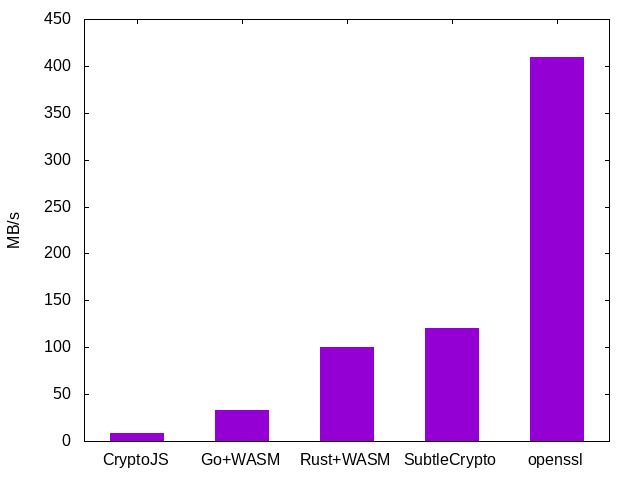
\includegraphics[width=0.7\linewidth]{images/hashingperformance.png}
        \caption{Hashing speed in MB/s (higher is better)}
        \label{fig:hashingperformance}
    \end{center}
\end{figure}


\subsection{Deciding On The In-Browser Hashing Implementation}
\label{subsec:deciding-on-the-in-browser-hashing-implementation}
It is clear from figure~\ref{fig:hashingperformance} that \texttt{SubtleCrypto} is the fastest of the options we tried.
Unfortunately, since it doesn't support piece-wise hashing we're forced to pick the next-fastest option,
the Rust-based implementation running in the \gls{WASM} \gls{VM}.
Using Rust provides us with another significant advantage:
the toolchain is highly developed.
Upon compilation, the toolchain auto-generates TypeScript declaration files containing the function signatures
the \gls{WASM} module exposes to the JavaScript world.
This is very nice, since it allows for compile-time type checking and for smarter code completion in the \gls{IDE},
as shown in figure~\ref{fig:dtside}.

\begin{figure}
    \begin{center}
        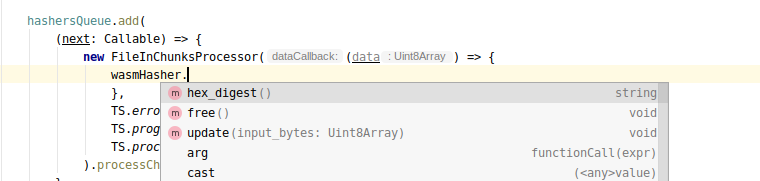
\includegraphics[width=0.7\linewidth]{images/dtside.png}
        \caption{Code Completion in Intellij}
        \label{fig:dtside}
    \end{center}
\end{figure}


\subsection{Software Libraries}\label{subsec:software-libraries}
Table~\ref{table:libraries} summarises the software libraries used in the implementation of the signing service.
All libraries we use are of high maturity, widely used, well tested and above all,
free and open source software.
That is, they are licenced with \gls{FSF} approved open source licences.

\begin{figure}
    \begin{center}
        \begin{tabular}{p{3cm}|p{12cm}}
            \textbf{Name} & \textbf{Description} \\ \hline
            logback &
            An implementation of the \gls{SLF4J} \gls{API}.
            It's a replacement for log4j, but brings a large number of improvements.
            Also, it's Swiss, which we found nice.
            We use it as the \gls{SLF4J} implementation.
            \\ \hline
            Apache HttpClient &
            Ktor's built-in \gls{HTTP} client isn't usable on its own,
            it requires a backing engine.
            We've selected the Apache HttpClient for this.
            Other alternatives were \gls{CIO}, Jetty, and OkHttp.
            It's probably the most configurable and complete \gls{HTTP} client available at the time of writing. It supports both \gls{HTTP}/1.1 and \gls{HTTP}/2,
            and is the only one available that supports following redirects and allows for configuration of timeouts and proxies.
            \\ \hline
            kotlinx.serialization &
            Kotlin Serialization is comparable to Jackson in that it provides serialisation of \gls{JSON},
            but unlike Jackson,
            it works without reflection.
            Instead it's implemented as a compiler plugin and a runtime library.
            The compiler plugin automatically generates the visitor code for the data classes,
            while the runtime library uses the generated code for serialisation without reflection.
            This massively improves runtime performance.
            \\ \hline
            JUnit &
            JUnit is probably the most widely used unit testing framework in the Java ecosystem.
            We use it to write our unit tests with it,
            as it provides convenient integration into Ktor.
            \\ \hline
            Bouncy Castle &
            Bouncy Castle is an extensive cryptography library for Java (and C\#).
            We use it extensively in the signing service:
            to build \gls{CMS} messages,
            to generate \gls{RSA} keys,
            to work with X.509,
            to create \gls{OCSP} and \gls{TimSP} requests and read the responses,
            and more.
            Without this library we couldn't have achieved what we did.
            Unfortunately, the documentation isn't very good (sometimes non-existent),
            and we've spent a lot of time figuring out how to use it correctly.
            \\ \hline
            auth0 jwt/jwks &
            Java implementations of the \gls{JWKS} and \gls{JWT} standards,
            used for \gls{OIDC} integration and id\_token verification.
            We haven't looked for alternatives because this library works well,
            has on-point documentation, and is MIT-licenced.
            \\ \hline
            jsoup &
            Jsoup is a library for working with \gls{HTML}.
            It provides a well-designed \gls{API} for extracting data from the \gls{DOM},
            using jquery-like methods.
            We use it to submit the login form on the Keycloack \gls{IDP} in the unit tests.
            We can't POST the form directly because there is a hidden \gls{CSRF} token field in the form,
            whose value we have to extract.
            This is what jsoup is good in.
            \\ \hline
            protobuf &
            This is the reference implementation of protocol buffers.
            We use it to build the signature file.
            \\ \hline
            Koin &
            Insert-Koin is a pragmatic, light-weight dependency injection framework for Kotlin.
            What distinguishes it from other \gls{DI} frameworks,
            and in our opinion makes it better,
            is that it uses purely functional resolution.
            There is no reflection, no proxies, and not even code generation.
            \\
        \end{tabular}
        \captionof{table}{Software libraries used in the development of the signing service\label{table:libraries}}
    \end{center}
\end{figure}

\subsection{Software Libraries - Verification Service}\label{subsec:software-libraries-verifier}
Table~\ref{table:libraries} summarises the software libraries used in the implementation of the verification service.
As with the libraries for the signing service,
they are all of high quality and free and open source software.
In some cases, we needed to fork and extend functionality for which we created pull requests in the respective project repositories.

\begin{figure}
    \begin{center}
        \begin{tabular}{p{4.2cm}|p{12cm}}
            \textbf{Name} & \textbf{Description} \\ \hline
            github.com/sirupsen/logrus & A structured logger, that is API compatible with the Go standard library logger. Used so we don't have to do the log formatting all by ourself. \\
            \hline
            go.mozilla.org/pkcs7 & Library for parsing and verifying \gls{PKCS7}/\gls{CMS} and RFC3161\cite{rfc3161} timestamps. \\
            \hline
            gopkg.in/square/go-jose.v2 & Implementation of the \gls{JOSE} set of standard like \gls{JWT} and \gls{JWK}. Used for extracting the X.509 certificates from the \gls{JWK}s in the signature data and for verifying the ID token signature. \\
            \hline
			github.com/coreos/go-oidc & Used for verifying and parsing the \gls{OIDC} ID tokens. \\
            \hline
            github.com/golang/protobuf & Reference implementation of protocol buffers, which are used in our signature format. \\
            \hline
            golang.org/x/crypto & Extended part of the Go standard library. Mainly used for parsing and verifying \gls{OCSP} responses. \\
            \hline
            github.com/shurcooL/vfsgen & Generates go "code" from static files and makes them accessible via a virtual filesystem. This is used to work around Go's limitation of not being able to embed files in the compiled binary.
        \end{tabular}
        \captionof{table}{Software libraries used in the development of the verification service\label{table:libraries-verifier}}
    \end{center}
\end{figure}

\subsubsection{Enhancing Mozilla's PKCS7 library with OCSP support}
Unfortunately, as useful as Mozilla's \gls{PKCS7} library is to us,
it doesn't support verifying \gls{OCSP} responses.
This is a bit of a surprise, as they are just \gls{CMS} messages themselves.
Since we needed the functionality,
we implemented this ourselves.
We will submit a pull request to Mozilla,
in the hope that they may find our contributions useful,
and if so, that they can include our contributions into their library.

\subsection{Dependency Management}\label{subsec:dependency-management}
For the signing service's dependency management,
we use Apache Maven~\cite{mvn}.
It allows us to specify project metadata,
build configuration,
and of course build- and runtime dependencies in a central location.
Most Java developers are familiar with Maven and should be able to feel right at home.
We chose Maven over alternatives such as Gradle and Ant because it is the most widely used dependency and build management system available in the Java world.

For the verifier,
we use Go's built-in module system.
A Go module is a set of Go packages in a file tree with a \texttt{go.mod} file at the root of the tree.
This file defines the dependency requirements,
which are pulled by the Go build system before compilation.
A Go package is included with an import path,
which specifies the location of the source code (the import path may be an \gls{URL}.
At this path the Go tool expects to find a source code repository (Git, SVN, Mercurial),
with the tagging system of the \gls{VCS} used for determining the version to use, if specified.

Unfortunately, in the web world, there are no such well thought out and coherent solutions,
and we are forced to combine multiple dependency management and build tools.
\paragraph{npm} The node package manager is used to install the TypeScript compiler \texttt{tsc},
which type-checks, then translates the TypeScript source code into JavaScript.
We also use \texttt{webpack},
a tool which allows us to combine all of the compiled JavaScript files into a single bundle file.
The code in that bundle file is minified,
a process in which the code is transformed in such a way as to be as small as possible.
This reduces the amount of data that has to be transmitted over the network.

\paragraph{Cargo} Cargo is the package manager for the Rust programming language.
It downloads dependencies, compiles packages,
and builds binaries ready for distribution.
We use Cargo to build the \gls{WASM}-based in-browser hashing binary,
which in turn is used by the frontend of the signing server as well as the verifier.

\subsection{Software Packaging}\label{subsec:software-packaging}
For the signing service,
we use the \texttt{shade} plugin for Maven.
This plugin allows us to package our artifact into a \gls{JAR},
including all runtime dependencies and resources.

For the signing server,
the resource files that have to be included into the production-ready \gls{JAR}
are the frontend files (\gls{HTML}, \gls{CSS}, \gls{JS} and \gls{WASM}),
as well as the Ktor configuration file.
This allows for simple deployment:
all that's needed on the target server is a \gls{JRE},
and the rest is contained in the \gls{JAR}.
The admin doesn't even have to set up Tomcat,
and running the server is as easy as executing \texttt{java -jar signingserver-shaded.jar}.

Go uses static linking by default,
it even includes its own \gls{VM} into the binaries it builds.
This has the advantage of vastly simplified deployment:
all anyone needs to do is to copy the binary and run it.
The downside is that the binary is somewhat larger.

However, Go's build system doesn't support including additional files in that single binary.
As a workaround, we've used the \texttt{vfsgen} library.
For a given set of files and directories represented as the \texttt{http.FileSystem} interface,
it generates Go code that statically implements that interface,
which in turn is used just like any other Go package.
The end result is one single executable file which contains everything it needs,
even its own runtime (unlike the fat \gls{JAR} which doesn't work without a \gls{JRE}).

\subsection{Custom Docker Image for Rust+Webpack Build}\label{subsec:custom-docker-image-for-rust+webpack-build}
Gitlab \gls{CI} uses docker images as the build environment in which to compile and package artifacts.
For all but one of our components we were lucky enough to find pre-built images providing what we needed (for example, a Maven 3 environment).
Unfortunately it seems with Rust + Webpack we're a bit on the forefront of things,
and no one's published a usable docker image for that build configuration to Dockerhub yet.

This is why we built our own image on top of a base Ubuntu+Rust image by adding the following:
\begin{enumerate}
    \item Installing \texttt{curl}
    \item Installing \texttt{wasm-pack}.
    This tool implements the workflow necessary for building Rust into \gls{WASM},
    generating the \gls{JS} and TypeScript binding code,
    and generates npm packages ready to be included into our project.
    \item Installing \texttt{cargo-generate}, a scaffolding tool which generates the boilerplate necessary for Cargo to work.
    \item Installing \texttt{npm}, the node package manager.
\end{enumerate}

We published this image onto Dockerhub as \texttt{izolight/rust-webpack},
hoping that others might find it useful.

\subsection{Combined Build Process}\label{subsec:combined-build-process}
Since we use so many languages, tools and frameworks,
the build process gets a bit complicated.
For this reason we document it here.

\begin{enumerate}
    \item \texttt{npm} downloads and installs the \texttt{webpack} and TypeScript toolchains
    \item \texttt{wasm-pack} calls \texttt{Cargo},
    which downloads and installs the Rust dependencies,
    and compiles the \gls{WASM} binaries
    \item \texttt{wasm-pack} generates glue code allowing for \gls{WASM} to \gls{JS} bindings
    \item \texttt{webpack} starts \texttt{tsc}, which typechecks,
    then translates the TypeScript source code into JavaScript.
    Then, it combines the generated \gls{JS} from \texttt{tsc} as well as \texttt{wasm-pack} into a minified bundle file,
    and packages it together with the \texttt{HTML} and \texttt{CSS} files.
    \item The verifier uses \texttt{go generate} to compile the frontend files it requires into a Go module,
    which were built in steps 1-4
    \item The signing server copies its frontend files built in steps 1-4 into its resources directory,
    then calls Maven to build its fat \gls{JAR}.
    \item The verifier calls \texttt{go build} three times,
    once respectively for GNU/Linux, Mac OSX and Windows,
    resulting in the binaries for each platform.
\end{enumerate}


Figure~\ref{fig:pipelines} illustrates the combined build process as implemented in Gitlab \gls{CI}.


\begin{figure}
    \begin{center}
        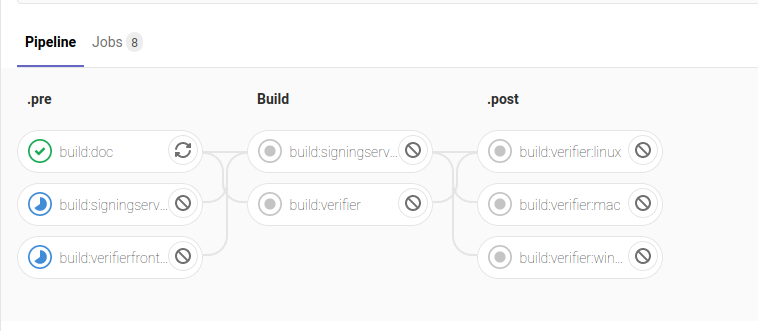
\includegraphics[width=0.7\linewidth]{images/pipelines.png}
        \caption{Gitlab CI pipelines combining different build tools and the artifacts they produce}
        \label{fig:pipelines}
    \end{center}
\end{figure}

\section{Implementation Components}\label{sec:implementation-components}
\subsection{Design Principles}\label{subsec:design-principles}
We've split the implementation of the Signing Service and the Verifier into small,
replaceable modules with clearly defined interfaces.
We've done this to achieve clear separation of concern and loose coupling,
in the spirit of the Law of Demeter~\cite{demeter}.

\paragraph{The Law of Demeter} is a well-known heuristic that states that any module should not know about the
internals of the objects it manipulates.
It is a special case of Loose Coupling.
Objects should hide their data, and expose operations.
This makes it easy to add new types of objects without requiring changing existing behaviours.
It also makes it hard to add new behaviours to existing objects.
Data structures should expose data and have no significant behaviour.

\paragraph{Loose Coupling} refers to the degree of knowledge that one component has of another.
Structuring programs to consist of components that know little of one another
results in easy-to-understand, easy-to-test code.
Developers new to the project can start with work on a small module and don't need to understand the whole system.
Refactoring (or replacing) the implementation of a component becomes easy,
as there are clear boundaries,
and changing the implementation of one component does not affect the others as long as
the boundary contract remains satisfied.


\paragraph{Inversion of Control} enables us to remove the few interdependencies remaining in the modules:
knowing about each other.
A component should not care about where, how and why another component is implemented,
it should only care about being provided the behaviour it requires.
Inversion of Control through Dependency Injection allows each component to declare
its dependencies through interfaces,
and having it supplied the implementation of that interface from the system it is part of,
without knowing anything whatsoever about that implementation.

Applying these methodologies doesn't guarantee clean code, nothing does.
However in our experience, modularisation, decoupling, and separation of concerns is the best single principle
to apply to software development to achieve some level of code quality.

\subsection{Components of the Signing Service}\label{subsec:modules-of-the-signing-service}
There are three groups of components in the signing service:
\begin{itemize}
    \item The views: They implement the \gls{REST} interface to the outside world.
    \item The services: Replaceable components providing functionality needed by the views in order to
    be able to meet their purpose.
    \item Marshalling: Classes which provide type-safe serialisation and de-serialisation of input and output data,
    as well as validation
\end{itemize}

\begin{figure}
    \begin{center}
        \begin{tabular}{p{4.2cm}|p{12cm}}
            \textbf{Name} & \textbf{Description}
            \\ \hline
            SigningKeysService &
            Generates signing keys and associated \gls{PKCS10} certificate signing requests,
            signs \gls{CMS} messages using the \gls{CA}-signed certificate and its key.
            The signing key never leaves this service.
            It can be backed by a \gls{HSM}.
            \\ \hline
            CAService &
            Provides an interface to the \gls{PKI} services offered by a \gls{CA}.
            It submits \gls{PKCS10} certificate signing requests to the \gls{CA} and returns the signed certificate.
            \\ \hline
            TimestampingService &
            Provides an interface to the RFC 3161 trusted timestamping services.
            Given the data to timestamp, it constructs a timestamping request (including a nonce for increased security),
            submits it, and returns the timestamping response.
            The response is a \gls{CMS} containing the signature of the hash of the data
            as well as the certificate chain of the signing certificate.
            \\ \hline
            OIDCService &
            Implements \gls{OIDC}-related functionality.
            An \gls{OIDC} client is configured using a discovery document usually located under \texttt{.well-known/openid-configuration}.
            Upon instantiation,
            this service fetches the discovery document as configured and set itself up.
            It validates \gls{JWT} id\_tokens,
            and it constructs authorisation endpoint \gls{URL}s for the frontend based on the discovery document.
            \\ \hline
            NonceGenerator &
            Generates nonce values in a secure manner.
            \\ \hline
            SecretService &
            Stores the static server secret used for authentication of the nonce values as described in~\ref{subsec:draft-1:-making-the-protocol-stateless},
            and operates on it.
            The server secret never leaves this service,
            and it could be backed by a \gls{HSM} or other hardware crypto device for increased security.
            At the moment, the secret is generated randomly at instantiation time, and not configurable nor persisted,
            for security.
            We would like to apologise for the pun, but we couldn't help ourselves.
        \end{tabular}
        \captionof{table}{Services and their responsibilities in the signing service\label{table:services}}
    \end{center}
\end{figure}

For a \gls{UML} component diagram showing a simplified overview of the components, see figure~\ref{fig:signingservicecomponents}.

\begin{figure}
    \begin{center}
        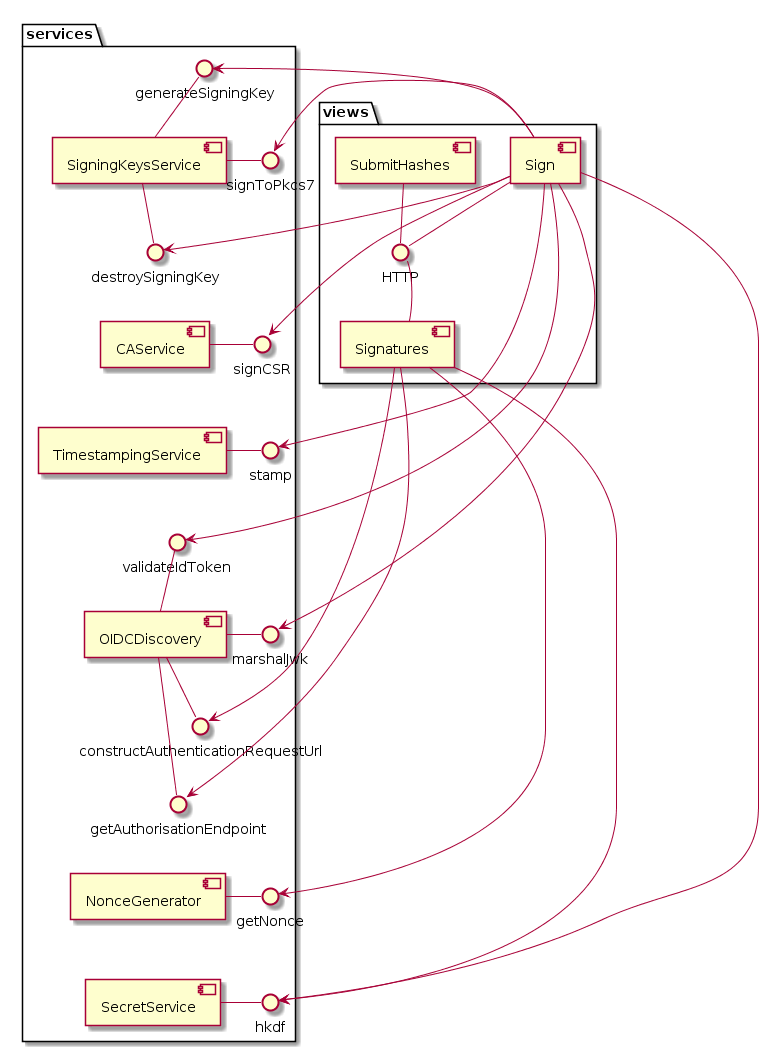
\includegraphics[width=0.7\linewidth]{images/signing_service_components.png}
        \caption{Signing Service Components}
        \label{fig:signingservicecomponents}
    \end{center}
\end{figure}


\subsection{Components of the Verifier}\label{subsec:modules-of-the-verifier}

The verifier is divided into the following packages:
\begin{itemize}
	\item verifier: Contains all the verifying logic. A detailed list with the components is below
	\item verifier/api: The http router is set up here together with the handlers.
	\item verifier/config: Configuration files (for now just our rootCA, which isn't in the system truststore), which will be embedded into the binary via vfsgen.
	\item verifier/static: The generated frontend files(html, js, wasm), which will be embedded into the binary via vfsgen.
	\item verifier/pb: The generated protobuf serialisation and some helper functions for pretty printing the values.
	\item verifier/cmd: The entrypoint with the main() function, which wires together the other packages and starts the web server.
\end{itemize}


\begin{figure}
	\begin{center}
		\begin{tabular}{p{4.2cm}|p{12cm}}
			\textbf{Name} & \textbf{Description}
			\\ \hline
			Verifier &
			Takes the outer deserialised protobuf file and the submitted hash and delegates the verifying of signature to the other verifier.
			All other verifiers will be started in go routines so they can start verifying as soon as possible.
			Some verifiers depend on output of other verifiers, which will be injected into them via calls from the main verifier that reads from or writes to channels in the other verifiers.
			It will finish either when one of the verifiers encounters an error or all of them have finished.
			\\ \hline
			TimestampVerifier &
			Parses the RFC 3161 timestamps and verifies them.
			If multiple timestamps are included, the outermost(last) timestamp timestamps the previous one until the innermost(first) contains the timestamp for the signature container.
			\\ \hline
			SignatureContainerVerifier &
			Verifies the \gls{PKCS7} which envelops our signature data.
			\\ \hline
			SignatureVerifier &
			Checks if the submitted hash is included in the salted hash list and if the list matches the ID token nonce.
			\\ \hline
			IDTokenVerifier &
			Verifies if the ID token is valid(just in a OIDC manner, our use of the nonce will be verified in the SignatureVerifier).
			\\ \hline
			LTVVerifier &
			Is called by the other verifiers to check if the included \gls{LTV} data (if any) verifies for the used certificates.
		\end{tabular}
		\captionof{table}{Services and their responsibilities in the verification service\label{table:services-verifier}}
	\end{center}
\end{figure}

For a \gls{UML} component diagram showing a simplified overview of the components, see figure~\ref{fig:verifiercomponents}.

\begin{figure}
    \begin{center}
        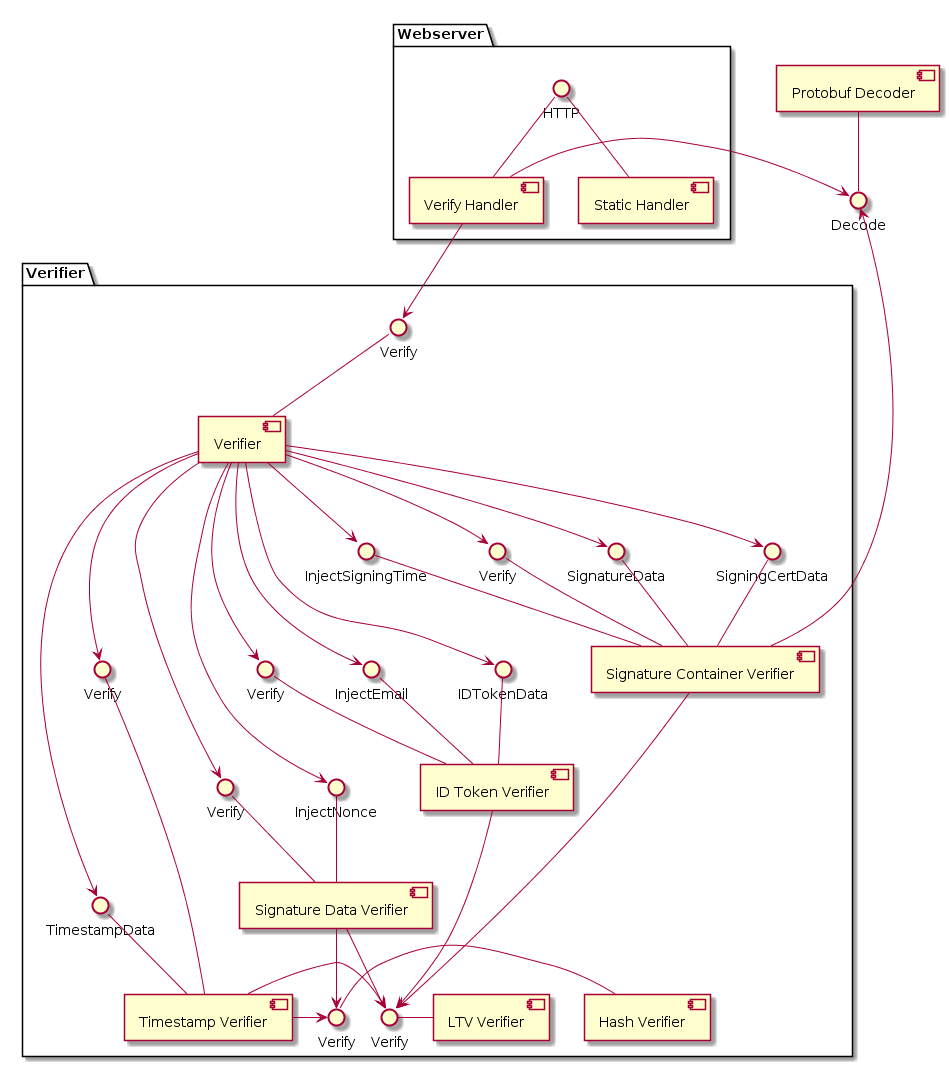
\includegraphics[width=0.7\linewidth]{images/verifier_components.png}
        \caption{Verifier Components}
        \label{fig:verifiercomponents}
    \end{center}
\end{figure}



\section{Finding services fitting our requirements}\label{sec:finding-services-fitting-our-requirements}

For our remote signing service to work,
we need an \gls{IDP} satisfying the requirements documented in section~\ref{sec:requirements-for-idps},
a \gls{TSA} willing to timestamp our signatures,
and a \gls{CA} with an \gls{OCSP} responder that will sign our certificates.

\subsection{Finding a TSA}\label{subsec:finding-a-tsa}
Searching for publicly available \gls{TSA}s, we've found a list as part of the software-library~\texttt{python3-rfc3161ng}~\cite{pythonrfc3161}:
\begin{itemize}
    \item \url{http://freetsa.org/tsr}
    \item \url{http://time.certum.pl}
    \item \url{http://timestamp.comodoca.com/rfc3161}
    \item \url{http://timestamp.geotrust.com/tsa}
    \item \url{http://timestamp.globalsign.com/scripts/timstamp.dll}
\end{itemize}

However we went with the SwissSign \gls{TSA}, as it seemed the least untrustworthy to us.

It worked as expected the first time we tried requesting a timestamp from it.
We used the \texttt{openssl ts} command line program.
Furthermore, to our knowledge, it is available free of charge,
and during our development and testing they didn't restrict us as to the number of timestamps we requested,
which was good enough for our \gls{POC}.

It can be found at \url{http://tsa.swisssign.net}.

We construct the timestamping requests using the \texttt{TimeStampRequestGenerator} class from BouncyCastle~\cite{timestamprequestgenerator},
which works well.

\subsection{Finding an IDP}\label{sec:finding-an-idp}
Finding an \gls{IDP} prividing such strong guarantees as required for Swiss citizens was not easy,
we were able to find only one: SwissID.
We searched online for documentation from them on how we could integrate their \gls{IDP} into our project,
but we could find none.
So we sent them an e-mail and asked, and got a phone call from one of their key account managers,
who seemed to understand little of our actual request but wanted to send us a whitepaper.
That turned out to be marketing material with very little technical information and quite useless to us.
Fearing the sudden appearance of a very large bill we stopped communicating with them.

For the purposes of our \gls{POC} and in the interest of having a working demo soon,
we don't really need an \gls{IDP} with actual guarantees, we just need any working \gls{OIDC} \gls{IDP}.

That led us to search for publicly available \gls{IDP}s that we could use free of charge,
with self-onboarding and readily-available online documentation.

We found the following:
\begin{itemize}
    \item Github: Doesn't support \gls{OIDC}, only OAuth
    \item Yahoo, Paypal, Salesforce, Phantauth, Okta, Google: Don't use X.509
    \item Microsoft: Uses X.509, but the intermediate certificate is self-signed. Why they're doing that is unclear to us, it seems futile.
\end{itemize}

So, in the end, unfortunately we didn't find a single free-of-charge \gls{IDP} that we could use.
Thus we were forced to set up our own.
For this purpose we selected Keycloak, a powerful \gls{IDM}, developed by Red Hat~\cite{keycloak}.
Keycloak is highly configurable and allowed us to run exactly the \gls{IDP} we needed.
For the duration of our thesis, it can be found at \url{https://keycloak.thesis.izolight.xyz/auth/realms/master/.well-known/openid-configuration}.

\subsubsection{Infrastructure setup for the IDP}
It would've been easy to run Keycloak on our local machines, and for the demo this would've been enough,
but we wanted to do it properly, with an internet-accessible \gls{IDP}.
To achieve this, we needed an internet-accessible server, a certificate for \gls{HTTPS},
and \gls{DNS} entries.

For the server, we chose Scaleway's development server simply because it costs as little as 3 EUR per month~\cite{scaleway}.
For certificates, we used the excellent Let's Encrypt \gls{CA}~\cite{letsencrypt}, which is a trusted \gls{CA} issuing domain validation certificates free of charge.

\begin{figure}
    \begin{center}
        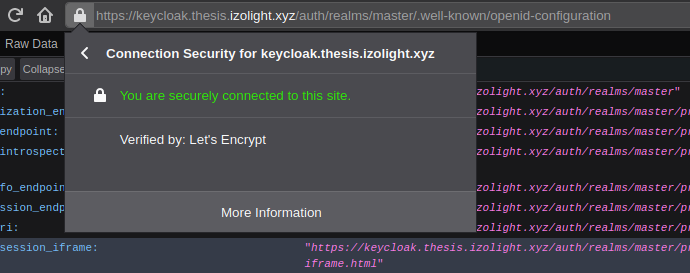
\includegraphics[width=0.7\linewidth]{images/firefox.png}
        \caption{Firefox trusting the certificate issued by the free and open CA Let's Encrypt}
        \label{fig:letsencrypt}
    \end{center}
\end{figure}

This only left us with \gls{DNS}.
Fortunately Gabor Tanz already runs his own \gls{DNS} server for other purposes (and also owns a domain),
so we simply added the appropriate subdomain entries and we were ready to proceed.


\subsection{Finding a CA}\label{subsec:finding-a-ca}
Unfortunately, Let's Encrypt doesn't issue signing certificates~\cite{letsencryptfaq}, only domain validation certificates.
We didn't spend much time searching for other \gls{CA}s since we expected to find none that issues
signing certificates in an automated way and free of charge.
Consequently we proceeded to set up our own \gls{CA}, as we did with the \gls{IDP}.
This meant more of an up-front investment of time,
but better predictability of efforts since everything would be under our control,
if we'd run into any issues.

To set up our own \gls{CA}, we selected Cloudflare's \texttt{cfssl} \gls{PKI} toolkit~\cite{cfssl}.
There was no evaluation of which software to use,
since at this point we were behind schedule
(because we spent more time on the concept part than we planned in order to get multi-signatures right).
We weren't keen on spending much more time on evaluating the \gls{CA} toolkit to use because it'd be relevant for the \gls{POC} only anyway,
and it didn't matter too much as long as it fulfilled its purpose.
On top of that we already had some knowledge of \texttt{cfssl}.

On the same server we'd already spun up to host our \texttt{Keycloak} \gls{IDP},
we installed \texttt{cfssl}.

\subsection{Real-time updating of OCSP responses for certificates issued}\label{subsec:real-time-updating-of-ocsp-responses-for-certificates-issued}
\texttt{cfssl} keeps a database of the certificates it issues,
which mainly consists of the subject name hash and the certificate's serial number.
Periodically, the \gls{OCSP} responder software checks the certificates issued,
and generates \gls{OCSP} responses for these certificates,
which it in turn stores in its own database.
This is done for perfomance reasons,
as generating an \gls{OCSP} response would be too costly.

Ordinarily this wouldn't be a problem, but for our purposes we need the \gls{OCSP} responses to be available immediately,
since we generate, sign and destory the signing key in a manner of seconds.
The fastest \texttt{cfssl} is able do update its \gls{OCSP} response database is once per minute,
which is way too slow for us.
Interactive users can't wait for 60+ seconds for signature generation.

So we expanded \texttt{cfssl}'s code to generate the \gls{OCSP} responses real-time,
that is, as soon as a certificate is issued and stored in the database,
the associated \gls{OCSP} response is generated and stored in the responders' database.

We have found many people on the internet asking for the same feature,
hitting the same problem we did.
For this reason we will submit a pull request to the \texttt{cfssl} project with our enhancements,
hoping that others might find it helpful.

\subsubsection{Separation of services using Docker containers}

In order to have some separation between the different pieces of software we decided to use Docker.
Furthermore docker makes the deployment of the software easier as we don't have to install software and their dependencies, which may conflict on the host system.

Table~\ref{tbl:docker} contains a complete list of Docker containers running on our server.
For a graphical representation, please see figure~\ref{fig:infrastructurebigpicture}.

%\paragraph{\texttt{traefik}} is an open-source edge router implementation.
\paragraph{traefik} is an open-source edge router implementation.
It receives outside requests on behalf of the actual system,
finds out which service is responsible to handle them,
and then passes them on.
It is able to automatically discover configuration and provide its routing accordingly,
and it can act as a \gls{HTTPS} termination point.
This helps lessen the load on backend components.
In our case, it takes \gls{HTTPS} requests, figures out which container is responsible for handling it,
and passes it on as \gls{HTTP} (thus terminating \gls{TLS}).


\paragraph{Keycloak} is the \gls{IDP}, and \texttt{keycloak-db} contains its PostgreSQL database.
\paragraph{cfssl-root} and \texttt{cfssl-intermediate} contain the respective root and intermediate certificates,
and serve certificate signing requests.
The containers with the \texttt{-db} suffixes run their PostgreSQL databases, same as for keycloak.
The intermediate \gls{CA} exposes a \gls{REST} \gls{API} used by the signing server.
\paragraph{cfssl-root-ocsp} and \texttt{cfssl-intermediate-ocsp} contain the \gls{OCSP} responders,
which handle \gls{OCSP} requests for certificates issued by \texttt{cfssl-root} and \texttt{cfssl-intermediate}.

\begin{figure}
    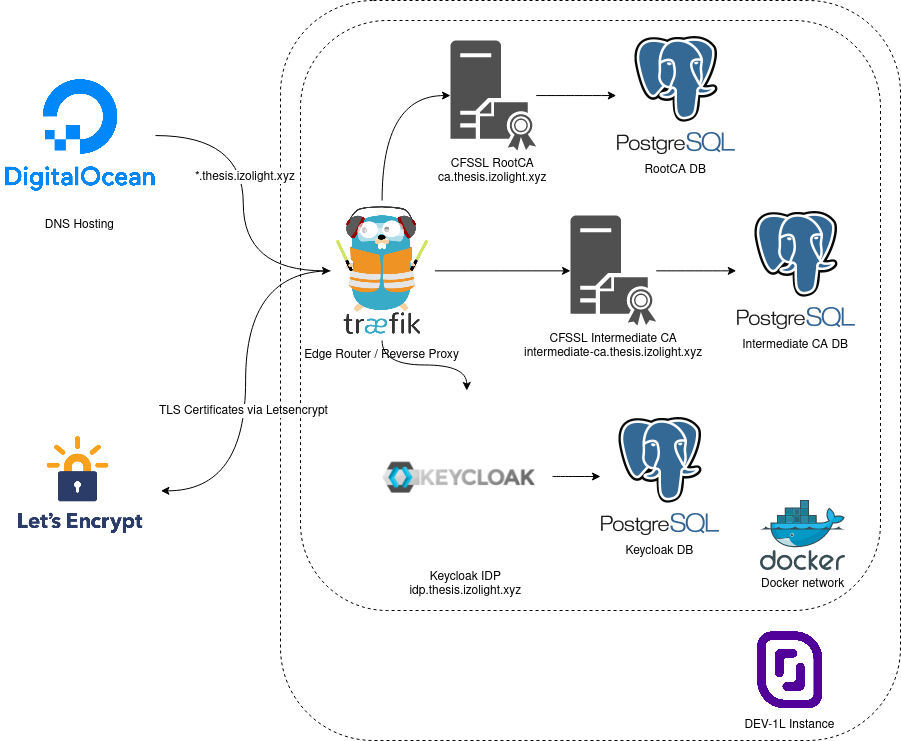
\includegraphics[width=0.9\linewidth]{images/infrastructure.png}
    \caption{Infrastructure Big Picture}
    \label{fig:infrastructurebigpicture}
\end{figure}

\begin{figure}
    \begin{center}
        \begin{tabular}{p{3.4cm}|p{5.7cm}|p{6.2cm}}
            \textbf{Name} & \textbf{Command} & \textbf{Ports} \\
            \hline
            traefik & /entrypoint.sh --docker\ldots & 0.0.0.0:80->80/tcp, 0.0.0.0:443->443/tcp \\*
            \hline
            keycloak & /opt/jboss/tools/docker-entrypoint\ldots & 127.0.0.1:8080->8080/tcp, 8443/tcp \\*
            \hline
            keycloak-db & docker-entrypoint.sh postgres & 5432/tcp \\*
            \hline
            cfssl-root & cfssl serve -db-config=/data/cfssl/\ldots & 8888/tcp \\*
            \hline
            cfssl-root-db & docker-entrypoint.sh postgres & 127.0.0.1:5432->5432/tcp \\*
            \hline
            cfssl-intermediate & cfssl serve -db-config=\ldots & 8888/tcp \\*
            \hline
            cfssl-intermediate-db & docker-entrypoint.sh postgres & 127.0.0.1:5433->5432/tcp \\*
            \hline
            cfssl-root-ocsp & cfssl ocspserve -address=0.0.0.0\ldots & 8888/tcp \\*
            \hline
            cfssl-intermediate-ocsp & cfssl ocspserve -address=\ldots & 8888/tcp \\*
        \end{tabular}
        \captionof{table}{Docker containers running on our POC server\label{tbl:docker}}
    \end{center}
\end{figure}

\section{Method of Work}\label{sec:method-of-work}
Two people hacking away at a shared project each on their own rarely works out well.
If we're lucky the code produced might even work, but it's probably going to be of low quality,
and there's risk of duplication of effort,
coordination and communication difficulties,
as well as exceeding deadlines.

This is why before starting work, we agreed upon a minimum of methodology.

\subsection{Version Control for Source Code}\label{subsec:version-control-for-source-code}
We put all source code under version control, in a shared repository.
This way each student can see what the other person is working on,
and the thesis advisors can keep an eye on what we're doing.
The commit log comes in handy for documenting the work timeline after the fact as well,
and it's a way of backing up our work.
Thankfully \gls{BFH} offers its students a Gitlab instance~\cite{gitlab}, so we will be using that.

\subsection{Standardised Build Tools and Environment}\label{subsec:standardised-build-tools-and-environment}
Few things are more annoying in a developer's life than troubleshooting build failures.
One developer adds a dependency, installs it on their machine, and forgets to tell the others.
Another developer updates their system and now uses a later version of a library, causing incompatibilities.

Furthermore,
our advisors most likely aren't very keen on installing the toolchains necessary for building our artefacts on their own machines,
they'd rather directly examine the results.

This is why a standardised, centralised build environment is a good thing to have.
Since \gls{BFH} is so kind as to offer us Gitlab runners toghether with their Gitlab instance~\cite{gitlab},
we will use that.
We've set up build pipelines based on Docker images to build our components as well as the documentation each time new commits are pushed to the master branch.
Figure~\ref{fig:gitlabcijobs} contains a screenshot of what this looks like in Gitlab's web interface.

\begin{figure}
    \begin{center}
        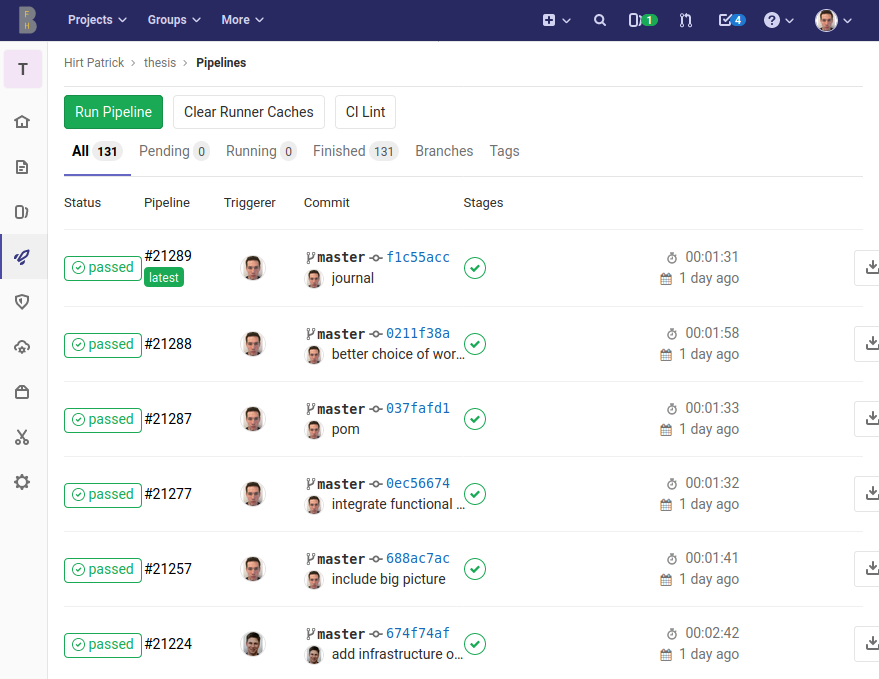
\includegraphics[width=0.8\linewidth]{images/gitlabcijobs.png}
        \caption{Gitlab CI Jobs}
        \label{fig:gitlabcijobs}
    \end{center}
\end{figure}

\subsection{Subdividing Work Packages}\label{subsec:subdividing-work-packages}
To be able to plan and schedule our work efficiently,
we divided the work packages into user stories,
as is customary in SCRUM.
We again used Gitlab for filing, planning and tracking the user stories.
Gitlab's issue system isn't exactly meant for use with SCRUM,
but we've managed to adapt it by using it as follows:
\begin{itemize}
    \item Issues are used for User Stories
    \item Labels are used for tracking progress ("todo", "doing", "done")
    \item Milestones are used for Sprint boundaries
\end{itemize}
Together with the issue board view used as a Storyboard view,
this works quite well for smaller projects such as ours.
Figure~\ref{fig:scrumboard} contains a screenshot of what this looks like.

\begin{figure}
    \begin{center}
        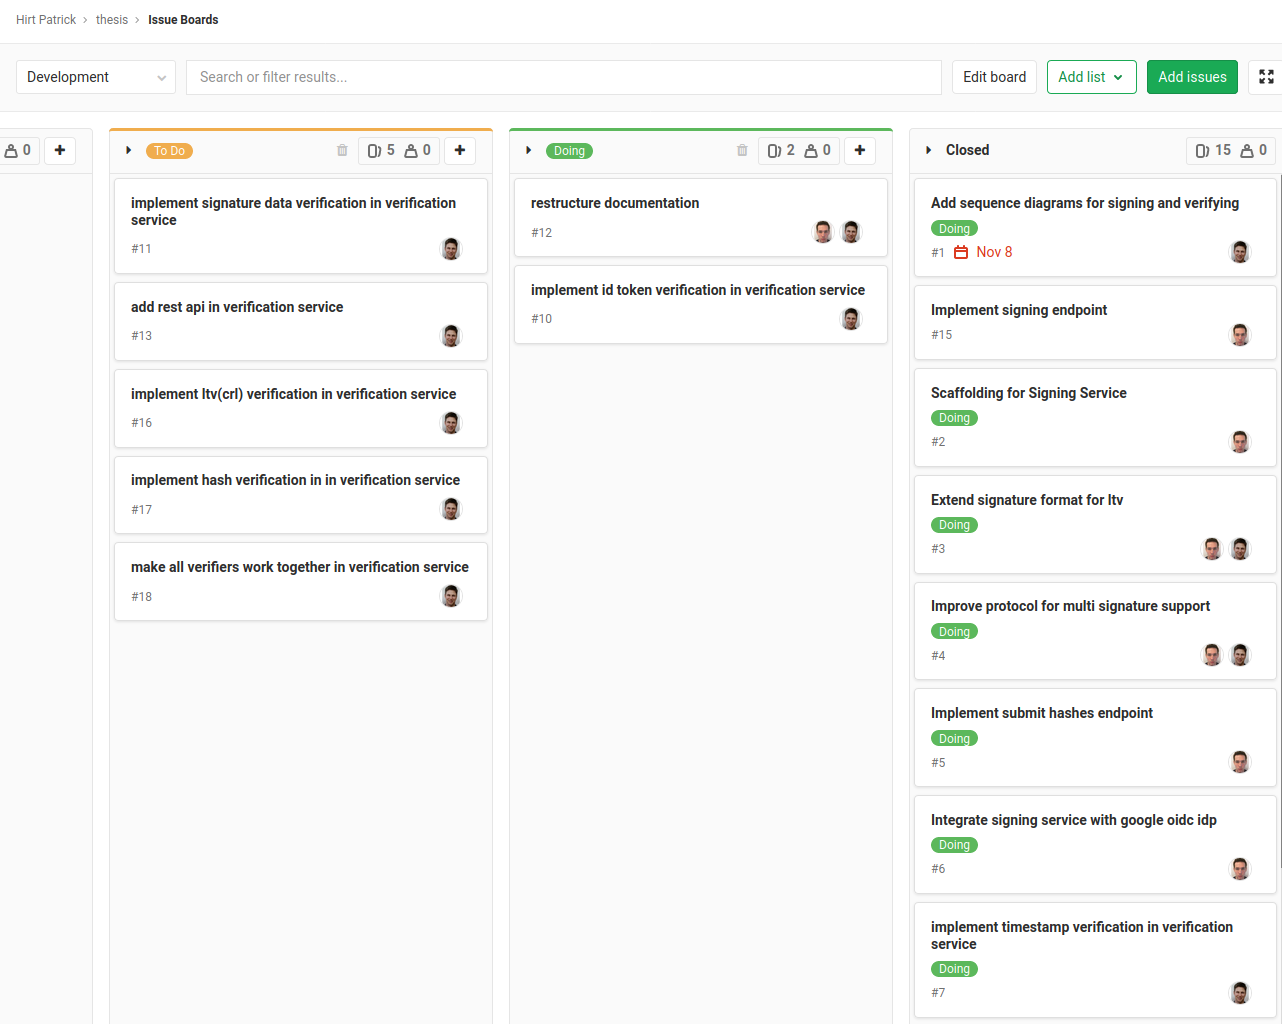
\includegraphics[width=0.8\linewidth]{images/board.png}
        \caption{SCRUM Storyboard}
        \label{fig:scrumboard}
    \end{center}
\end{figure}

\subsection{Tracking Progress}\label{subsec:tracking-progress}
In addition to the commit log and the Storyboard,
we kept an informal work log in the repository so that our advisors can check up on our progress effortlessly
any time they want.
On top of that we met with them regularly during the whole work,
discussing the progress, potential issues and of course to receive regular feedback.

\subsection{Test Coverage}\label{subsec:test-coverage}
For the signing server, we achieve a test coverage of 86.4\%,
as measured by the Intellij coverage runner.
This value, while respectable, isn't that as high as we'd like.
We inspected the coverage report and found that this is mainly due to deserialisation code in data classes that must take fields that are never used.
Excluding these classes, we achieve a coverage of 94.9\%.

For the verification server, we achieve a test coverage of 85.3\%,
as measured by the Go test tool.
Most of the uncovered parts are due to the same reasons as in the signing server tests.




\chapter{CSC Standard}\label{ch:cscstandard}

\section{CSC Specification}\label{sec:csc-specification}

The \acrfull{CSC} has been formed to standardise cloud-based digital signatures, while meeting the \gls{EU}'s regulation for signatures (\gls{eIDAS}).
The consortium consists of of all kind of members from different industries: Software companies like Adobe,
the German Bundesdruckerei, Certificate Authorities (\gls{CA}) like QuoVadis,
but also academic institutions like the Technische Universit\"at Graz.

The result of this consortium is an \gls{API} specification for remote electronic signatures and remote electronic seals.
The specification is published as a \gls{PDF} document, as well as an \gls{OpenAPI} specification, and a \gls{JSON} schema~\cite{csc-spec}.


\subsection{Comparison}\label{subsec:comparison}
We have examined the standard and compared it to our solution.
We document the findings in this section.

\subsubsection{Information Leakage to IDP}

One main difference is that in the \gls{CSC} specification,
the \gls{IDP} gets to know the hash that will be signed,
and how many documents will be signed through the \texttt{numSignatures} and hash parameters in the credential authorisation,
which has a slight impact on privacy and is a violation of the least information principle.
In our solution, this problem doesn't exist.

\subsubsection{Information Leakage to Signing Service}
The \gls{CSC} standard allows for the document to be signed to be transmitted to the signing service.
We see absolutely no reason at all for this to be allowed,
since in any case,
only a hash of the document is signed.
There is no scenario - be it in our solution, or Adobe's - where the signing service is required to recieve the full document.
This is a violation of the least information principle and a break of privacy.
In our solution, this problem doesn't exist.

\subsubsection{Missing Separation of Concern}
The \gls{CSC} standard allows for the \gls{IDP} and the signing service to be the same system,
controlled by the same organisation.
We find this highly problematic, as this means a single entity is able control all the parts needed to create a signature.
To be fair, the \gls{EU} allows this as well.
We strongly disagree with this, and explicitly forbid it in our specification.
There should never be a single organisation in complete control, especially not one with a profit motive.

\subsubsection{Weak Authentication}
The \gls{CSC} standard allows for \gls{HTTP} Basic or Digest authentication.
Saying this is wholly inadequate for creating legally binding signatures would be an understatement.

\subsubsection{No Use of Standard Protocols}
The \gls{CSC} standard doesn't use standard protocols like \gls{OIDC} or even \gls{SAML},
which is a disadvantage:
Before any \gls{IDP} can be used, it has to implement the extensions specified by the \gls{CSC} standard.

Another difference is that a \gls{SAD} is returned to the client,
which has a defined validity period and allows for further signatures to be created without re-authorisation,
which means that an attacker who is able to steal the \gls{SAD} could sign arbitrary documents.
In our solution, this isn't possible.

\subsubsection{No User Controlled Signing Process}
With the \gls{CSC} standard, there is nothing stopping the \gls{TSP} creating signatures without the user's knowledge or consent.
The \gls{TSP} controls all parts necessary.
The \gls{SAD} looks good on paper,
as it suggests the user is in control of their key,
but in reality there is no security whatsoever to it.
In our solution, the signing service cannot create a signature without the direct authorisation of the user through the \gls{IDP},
which we forbid to be controlled by the same organisation.

\section{Conclusion}\label{sec:conclusion}
We find the \gls{CSC} standard to be significantly less secure than our proposal.
There are significant privacy and security issues.
Personally, we would not use any solution based on this standard.

\chapter{Yubikey HSM}

In a first look at the yubikey hsm and the required packages we found that the access for the developer always happens via the yubikey-connector which provides a http server.
The protocol however is not documented and is binary. The developer always has to go through libyubihsm to connect with the server.
From this we can conclude that the intended use is to have the yubikey hsm on a device with just the connector running and nothing else and the application interfacing with the hsm on another server.
This scenario would improve security as the application doesn't have direct hardware access to the hsm.
\chapter{Further Work}\label{ch:further-work}
Due to time constraints given by the timeboxed bachelor thesis, we weren't able to explore all aspects of the remote signing service.
We document these aspects and our thoughts on them here for future works.

\section{Public Append-Only Data Structure}\label{sec:public-append-only-data-structure}
The main defence against malicious signature services - signing document files without the users' consent - is the integration of the authentication token signed by the \gls{IDP} into the signature file TODO link to section where this is explained in more detail.
If the signing server were to create a signature file on their own they'd be unable to get such a token from the \gls{IDP}, and this would be detected upon signature verification.

However, if the \gls{IDP} were under the control of the same organisation as the signing service,
or if the \gls{IDP} were compromised as well,
or if the user were to be tricked into authenticating with the \gls{IDP} not knowing what they were doing,
a malicious signing service could still create a valid signature not authorised by the user.

In order to defend against this, as an additional safety mechanism, we propose using a public append-only data structure,
inspired by blockchain technologies.
The signature service would be required to publish all signatures it creates by appending them to this data structure.
This would allow everybody and anybody to see the signatures the signing server issues.

If the signing service were to create a signature without the users' consent,
the signer could see this by inspecting the data structure,
as there would be an entry for a signature there the signer doesn't remember creating.

If the signing service were to create a signature without publishing it into the data structure,
everyone could see this by inspecting the data structure,
because the signature file would not be published in it.


\section{Multi-Party Signatures}\label{sec:multi-party-signatures}
In order to facilitate signatures with multiple parties (for example, a standard apartent rental contract) we need to design a mechanism for generating and validating such signature schemes.
There are many possibilities to implement this.

\subsection{Nested Signatures}
One possibility is that the next signer signs the previously created signature file of the document instead of the document itself.
The signing service will then generate another signature for the previous signature.
The new signature would replace the original one, as it embeds it.
This can be repeated as many times as necessary, creating a chain of signatures.
This method would allow not only for an arbitrary number of signatures on the same document,
but it would also embed ordering of the signatures.
This could be useful, as some organisation's processes may require their documents to be signed in a specific order.

For the validation process just the final signature is needed (as it embeds all previous signatures) and the document itself,
and then the whole signature chain can be validated recursively,
with the innermost signature validating the document integrity.

\subsection{Pairing-based Signatures}
With pairing-based cryptography like \gls{BLS}~\cite{bls} we could implement n-of-n or m-of-n multi signatures.
This wouldn't provide nor require any ordering in the signing process, and while much more elegant,
would complicate the cryptographic aspect\footnote{Saying we fully understand the mathematics behind it would be a lie.} and could introduce errors as we don't have a lot experience with pairing based cryptography.

\section{CADES Signatures}\label{sec:cades-signatures}
TODO supporting CMS/CADES signatures as defined in \url{https://www.etsi.org/deliver/etsi_ts/101700_101799/101733/02.02.01_60/ts_101733v020201p.pdf}
for inclusion in pdfs
%---------------------------------------------------------------------------

% Selbständigkeitserklärung
%---------------------------------------------------------------------------
\cleardoublepage
\phantomsection
\addcontentsline{toc}{chapter}{Declaration of authorship}
\chapter*{Declaration of primary authorship}
\label{chap:declaration_authorship}

\vspace*{10mm} 

I / We hereby confirm that I / we have written this thesis independently and without using other sources and resources than those specified in the bibliography. All text passages which were not written by me are marked as quotations and provided with the exact indication of its origin. 

\vspace{15mm}

\begin{tabbing}
xxxxxxxxxxxxxxxxxxxxxxxxxxxxxx\=xxxxxxxxxxxxxxxxxxxxxxxxxxxxxx\=xxxxxxxxxxxxxxxxxxxxxxxxxxxxxx\kill
Place, Date:		\> [Biel/Burgdorf], \versiondate \\ \\ 
Last Name/s, First Name/s:	\> [Test Peter] 	\> [M\"uster R\"os\"a] \\ \\ \\ \\ 
Signature/s:	\> ......................................\> ...................................... \\
\end{tabbing}

%---------------------------------------------------------------------------

% Glossary
%---------------------------------------------------------------------------
\cleardoublepage
\phantomsection
\addcontentsline{toc}{chapter}{Glossay}
%\renewcommand{\glossaryname}{Glossay}
\printglossary
%---------------------------------------------------------------------------

% Bibliography
%---------------------------------------------------------------------------
\cleardoublepage
\phantomsection
\addcontentsline{toc}{chapter}{Bibliography}
\bibliographystyle{IEEEtranS}
\bibliography{database/bibliography}{}
\printglossaries
%---------------------------------------------------------------------------

% Listings
%---------------------------------------------------------------------------
\cleardoublepage
\phantomsection
\addcontentsline{toc}{chapter}{List of figures}
\listoffigures
\cleardoublepage
\phantomsection
\addcontentsline{toc}{chapter}{List fo tables}
\listoftables
\lstlistoflistings
%---------------------------------------------------------------------------

% Index
%---------------------------------------------------------------------------
\cleardoublepage
\phantomsection
\addcontentsline{toc}{chapter}{Index}
    \printindex
    %---------------------------------------------------------------------------

    % Attachment:
    %---------------------------------------------------------------------------
    \appendix
    \settocdepth{section}
%    \chapter*{APPENDICES}
\addcontentsline{toc}{chapter}{APPENDICES}

\begingroup\let\clearpage\relax
\chapter{Arbitrary Appendix}
\label{chap:appendix_arb}
\endgroup

The European languages are members of the same family. Their separate existence is a myth. For science, music, sport, etc, Europe uses the same vocabulary. The languages only differ in their grammar, their pronunciation and their most common words. Everyone realizes why a new common language would be desirable: one could refuse to pay expensive translators. To achieve this, it would be necessary to have uniform grammar, pronunciation and more common words. If several languages coalesce, the grammar of the resulting language is more simple and regular than that of the individual languages. The new common language will be more simple and regular than the existing European languages. It will be as simple as Occidental; in fact, it will be Occidental. 
%    \chapter{Additional Appendix}
\label{chap:appendix_B}

\section{Test 1}
To an English person, it will seem like simplified English, as a skeptical Cambridge friend of mine told me what Occidental is. The European languages are members of the same family. Their separate existence is a myth. For science, music, sport, etc, Europe uses the same vocabulary. The languages only differ in their grammar, their pronunciation and their most common words. Everyone realizes why a new common language would be desirable: one could refuse to pay expensive translators. To achieve this, it would be necessary to have uniform grammar, pronunciation and more common words. If several languages coalesce, the grammar of the resulting language is more simple and regular than that of the individual languages. The new common language will be more simple and regular than the existing European languages. 

\subsection{Environment}
It will be as simple as Occidental; in fact, it will be Occidental. To an English person, it will seem like simplified English, as a skeptical Cambridge friend of mine told me what Occidental is. The European languages are members of the same family. Their separate existence is a myth. For science, music, sport, etc, Europe uses the same vocabulary. The languages only differ in their grammar, their pronunciation and their most common words. Everyone realizes why a new common language would be desirable: one could refuse to pay expensive translators. To achieve this, it would be necessary to have uniform grammar, pronunciation and more common words.
%    \chapter{Content of CD-ROM}
\label{chap:appendix_CDROM}

Content of the enclosed CD-ROM, directory tree, etc.
    \chapter*{APPENDICES}
\addcontentsline{toc}{chapter}{APPENDICES}

\begingroup\let\clearpage\relax
\chapter{Web Server from Go's Standard Library}
\label{chap:appendix_golangwebserver}
\endgroup

\begin{lstlisting}[language=Go]
package main

import (
    "log"
    "net/http"
)

func main() {
    log.Print("listening on :8080")
    log.Fatal(http.ListenAndServe(":8080", http.FileServer(http.Dir("."))))
}
\end{lstlisting}


    \chapter{Source Code for In-Browser Hashing}\label{ch:in-browser-hashing-code}

\section{Golang}\label{sec:golang}

\begin{lstlisting}[language=Go]
    package main

    import (
    "crypto/sha256"
    "fmt"
    "syscall/js"
    "time"
    )

    var hasher = sha256.New()
    var start time.Time

    func registerCallbacks() {
    js.Global().Set("progressiveHash", js.FuncOf(progressiveHash))
    js.Global().Set("startHash", js.FuncOf(startHash))
    js.Global().Set("getHash", js.FuncOf(getHash))
    }

    func progressiveHash(this js.Value, in []js.Value) interface{} {
    array := in[0]
    buf := make([]byte, array.Get("length").Int())
    js.CopyBytesToGo(buf, array)
    hasher.Write(buf)
    return this
    }

    func startHash(this js.Value, in []js.Value) interface{} {
    start = time.Now()
    fmt.Printf("Start: %s\n", start.Format(time.RFC3339Nano))
    hasher = sha256.New()
    return this
    }

    func getHash(this js.Value, in []js.Value) interface{} {
    hash := hasher.Sum(nil)
    hashStr := fmt.Sprintf("%x", hash)
    fmt.Printf("Hash: %s\n", hashStr)
    end := time.Now()
    fmt.Printf("End: %s\n",end.Format(time.RFC3339Nano))
    fmt.Printf("Took %s\n", end.Sub(start))

    return js.ValueOf(hashStr)
    }

    func waitForever() {
    c := make(chan struct{}, 0)
    <-c
    }

    func main() {
    fmt.Println("WASM Go Initialized")
    registerCallbacks()
    waitForever()
    }
\end{lstlisting}


\section{Rust}

\begin{lstlisting}[language=Rust]
    extern crate sha2;
    extern crate wasm_bindgen;

    use std::cell::Cell;
    use std::string::String;

    use sha2::Digest;
    use sha2::Sha256;
    use wasm_bindgen::prelude::*;

    #[wasm_bindgen]
    pub struct Sha256hasher {
    hasher: Cell<Sha256>,
    }

    #[wasm_bindgen]
    impl Sha256hasher {
    #[wasm_bindgen(constructor)]
    pub fn new() -> Sha256hasher {
    Sha256hasher {
    hasher: Cell::new(Sha256::default()),
    }
    }

    pub fn update(&mut self, input_bytes: &[u8]) {
    let hasher = self.hasher.get_mut();
    hasher.input(input_bytes)
    }

    pub fn hex_digest(&mut self) -> String {
    let hasher = self.hasher.take();
    let output = hasher.result();
    self.hasher = Cell::new(Sha256::default());
    return format!("{:x}", output);
    }
    }
\end{lstlisting}

\section{Reading a file piece-wise in TypeScript}
\begin{lstlisting}[language=Javascript]

interface FileChunkDataCallback {
(data: Uint8Array): void
}

interface ErrorCallback {
(message: string): void
}

interface FileReaderOnLoadCallback {
(event: ProgressEvent): void
}

interface ProgressCallback {
(percentCompleted: number): void
}

interface ProcessingCompletedCallback {
(startTime: Date, endTime: Date, fileSize: number): void
}


class FileInChunksProcessor {
public readonly CHUNK_SIZE_IN_BYTES: number = 1024 * 1000 * 20;
private readonly fileReader: FileReader;
private readonly dataCallback: FileChunkDataCallback;
private readonly errorCallback: ErrorCallback;
private readonly processingCompletedCallback: ProcessingCompletedCallback;
private readonly progressCallback: ProgressCallback;
private start: number = 0;
private end: number = this.start + this.CHUNK_SIZE_IN_BYTES;
private startTime?: Date;
private numChunks: number = 0;
private chunkCounter: number = 0;
private inputFile: File | null = null;

constructor(dataCallback: FileChunkDataCallback,
errorCallback: ErrorCallback,
progressCallback: ProgressCallback,
processingCompletedCallback: ProcessingCompletedCallback) {
this.fileReader = new FileReader();
this.fileReader.onload = this.getFileReadOnLoadHandler();
this.dataCallback = dataCallback;
this.errorCallback = errorCallback;
this.processingCompletedCallback = processingCompletedCallback;
this.progressCallback = progressCallback;
}

public processChunks(inputFile: File) {
this.inputFile = inputFile;
this.startTime = new Date();
this.numChunks = Math.round(this.inputFile.size / this.CHUNK_SIZE_IN_BYTES);
this.read(this.start, this.end);
}

public getFileFromElement(elementId: string): File | undefined {
const filesElement = q(elementId) as HTMLInputElement;

if (Validate.notNull(filesElement.files)) {
if (filesElement.files.length < 0) {
this.errorCallback("Too few files specified. Please select one file.")
} else if (filesElement.files.length > 1) {
this.errorCallback("Too many files specified. Please select one file.")
} else {
return filesElement.files[0];
}
}
}

private getFileReadOnLoadHandler(): FileReaderOnLoadCallback {
return () => {
if (Validate.notNull(this.inputFile)) {
this.dataCallback(new Uint8Array((this.fileReader.result as ArrayBuffer)));

this.start = this.end;
if (this.end < this.inputFile.size) {
this.chunkCounter++;
this.end = this.start + this.CHUNK_SIZE_IN_BYTES;
this.progressCallback(
Math.round((this.chunkCounter / this.numChunks) * 100));
this.read(this.start, this.end);
} else {
if (Validate.notNullNotUndefined(this.startTime)) {
this.processingCompletedCallback(
this.startTime, new Date(), this.inputFile.size);
}
this.progressCallback(100);
}
}
}
}

private read(start: number, end: number) {
if (Validate.notNull(this.inputFile)) {
this.fileReader.readAsArrayBuffer(this.inputFile.slice(start, end));
}
}

function errorHandlingCallback(message: string) {
const errorElement = q("error");
errorElement.innerHTML = `${errorElement.innerHTML} <p>${message}</p>`;
}

function progressCallback(percentCompleted: number) {
if (percentCompleted == 100) {
q("progress").innerText = `Completed!`
} else {
q("progress").innerText = `Hashing: ${percentCompleted}%`
}
}

export function processFileButtonHandler(wasmHasher: Sha256hasher) {
const startElement = q("start");
const startTime = new Date();
startElement.innerText = "started at " + dateObjectToTimeString(startTime);

const processor = new FileInChunksProcessor((data) => {
wasmHasher.update(new Uint8Array((data)));
},
errorHandlingCallback,
progressCallback,
(startTime, endTime, sizeInBytes) => {
const hashStr = wasmHasher.hex_digest();
wasmHasher.free();
}
);
const file = processor.getFileFromElement("file");
if (Validate.notNullNotUndefined(file)) {
processor.processChunks(file);
}
}
\end{lstlisting}

    %---------------------------------------------------------------------------

    %---------------------------------------------------------------------------
\batchmode
\end{document}

